\title{Sparse neural networks of exclusive coincidence classes}
\author{Aleksander Mendoza}

\documentclass[12pt]{article}
\usepackage{tikz}
\usepackage[utf8]{inputenc}
\usepackage[T1]{fontenc}
\usepackage{lmodern}
\usepackage{amsfonts}
\usepackage{mathrsfs}
\usepackage{centernot}
\usepackage{listings}
\usepackage{mathtools}
\usepackage{xcolor}
\usepackage{amsthm}
\usepackage{amsmath}
\usepackage{amssymb}
\usepackage{tikzit}
\usepackage{tabularx}
\usepackage{enumitem}
\input{style.tikzstyles}
\DeclareMathOperator*{\argmax}{argmax}
\DeclareMathOperator*{\argmin}{argmin}
\newtheorem{definition}{Definition}
\newtheorem{theorem}{Theorem}[section]
\newtheorem{corollary}{Corollary}[theorem]
\newtheorem{lemma}[theorem]{Lemma}
\renewcommand{\labelenumii}{\theenumii}
\renewcommand{\theenumii}{\theenumi.\arabic{enumii}.}
\begin{document}
\maketitle
\lstset{
	basicstyle=\ttfamily,
	mathescape
}


\begin{abstract}
We present a new model of neural networks that was inspired by an attempt to combine predictive coding and variational inference with sparse population coding and neural assembly calculus. This new approach can be used to learn extremely sparse and robust multi-layer networks without backpropagation or any error feedback whatsoever. It fits well with all biological constraints and leads to an emergence of receptive fields similar to those observed in neuroscience. It can be used to design biologically plausible convolutional networks without weight sharing. They are capable of extracting interdependent hierarchies of features, broadly similar to capsule networks proposed by Geoffrey Hinton. The networks learn from very little data and do not overfit. Due to high sparsity, their training and evaluation are extremely efficient (model with a few million weights can be trained efficiently even on a single thread). 
Just like human brain, our networks take advantage of motor feedback during learning in order to build semantic models of the data. This could potentially allow for building efficient reinforcement learning agents in the future. Thanks to immense sparsity, these networks have the potential of solving catastrophic forgetting problem with help of pattern separation (although empirical experiments are yet to be done). Our model does not fit functions like deep nets, but instead builds semantic graphs similar to hippocampus, which in theory could be used to infer group actions on data and allow for few-shot reinforcement learning (although empirical experiments are yet to be done).
\end{abstract} 


\tableofcontents 

\section{Introduction}

\paragraph{How to read this paper}

This paper is still work-in-progress. It contains complete details of all the results and conclusions that I reached. Reading all of it is not necessary. Every paragraph has some title that summarises its contents. Perhaps the most important points to takeaway are 
\begin{itemize}
	\item Convolutional networks can arise from image translation caused by eye movement (without the need for sharing weights)
	\item Deep networks achieve great results because they exploit function equivariances under certain group actions. Those group actions are ``hard-coded'' directly in the architecture. Our networks on the other hard try to learn those group actions by observing motor feedback. In short deep nets approximate functions, while ECC nets approximate groups.
	\item The receptive fields of grid cells are group cosets, when you treat movement in space as a translation group. Place cells are individual elements of the group relative to some ``anchoring points''. For example in one-dimensional space $(\mathbb{N},+)$ generated by ``agent actions'' $+1,-1$, the grid cells would be cosets $\mathbb{N}+0,\mathbb{N}+1,...,\mathbb{N}+n-1$ under $\mathbb{N} \mod n$ equivalence (where $n$ is the scale of compressed space representation) .
	\item The receptive fields of neurons could be seen as ``eigendinstributions'', whose linear combination determines the probability of every input stimulus  (with scalar coefficients being firing probabilities of respective neurons).
	\item Some people (including Geoffrey Hinton) have hypothesised existence of voting mechanism in cortical columns. Such ``voting-like'' behaviour can naturally emerge in our networks by adding recurrent connections.
	\item Our networks are a type of spiking networks, but their underlying theory works no matter whether the time is discrete or continuous.
	\item Reinforcement learning has trouble with sample efficiency. Deep nets are efficient because they exploit symmetries in data. We are missing networks that could exploit symmetries in actions, by treating the set of actions as a generator set of some group. For example head direction cells represent the rotational symmetry  $\alpha + 360^{\circ} = \alpha$. There should exist other types of cells that represents other group symmetries in action space. Building a human/animal-like reinforcement learning agents would solve sample efficiency problem and allow for greater generalisation by inferring those group symmetries from motor feedback.
\end{itemize}

\paragraph{Motivation}
Deep learning had its origins in an attempt to model biological neurons. Belief networks, Boltzmann and Helmholtz machines tried to capture the essence of neural computations using graphical models. A biological neuron could be interpreted as a node $f$ in some graph. Such nodes have binary values. When a neuron fires, the node holds value of $f=1$, otherwise it's $f=0$. Perceptron, predictive coding and variational inference work on a higher level of abstraction and instead of modelling individual spikes, they focus on estimating their frequency, also known as firing rate. ECC networks operate on sparse populations and individual spikes.



Consider a binary vector $\boldsymbol{x}$. Every single bit $x_i$ represents certain observation, such as for example a pixel ($0=$white, $1=$black). Every possible configuration of bits in $\boldsymbol{x}$ has certain probability $p(\boldsymbol{x})$. Individual bits are often not independent of each other. Learning the joint probability $p(\boldsymbol{x})$ is challenging and often inefficient. That's why restricted Boltzmann machines are more practical than their unrestricted counterparts. Throughout the history of deep learning, the common trick was to assume that the bits independent anyway. Then consecutive deeper layers could reconstruct the interactions between inputs. Nonetheless, within the same layer of the neural network, the value of every neuron is computed independently of the others. 

We introduce a new and fundamentally different approach, called the exclusive coincidence classes (ECC). The data obtained by performing observations and measurements of the real world, often contains hidden structure, which introduces correlations of various features. Suppose there are $y_1,y_1...y_n$ distinct ``events''
that may occur in the observed world and each of them manifests in its own way.

\paragraph{Introductory example}
Going back to the example of $\boldsymbol{x}$ being pixels, we might image observing a straight metal bar. As we observe this bar rotate in front of our eyes, it will cast a line-shaped shadow on our retina. We might choose to treat different  rotations as distinct ``events'' and use $y_1...y_4$ to denote the angles $0^{\circ},45^{\circ},90^{\circ},135^{\circ}$ respectively. We can infer the rotation $\boldsymbol{y}$ from observations $\boldsymbol{x}$ by building a simple neural network with only a single densely connected linear layer. The training could be achieved using softmax and backpropagation. This is not what exclusive coincidence classes would do. 

Notice that all of the explanations $\boldsymbol{y}$ are mutually exclusive.
The bar cannot exist in two positions simultaneously. It could potentially lie somewhere in between angles $0^{\circ}$ and $45^{\circ}$, and then we might be tempted to proportionally assign some fractional values to $y_1$ and $y_2$. This  has been the dominant approach taken by the deep neural networks so far, but the biological neurons are noisy and unreliable. They could never operate with enough precision to pick up on such fractions. This is the reason why predictive coding has been forced to explain everything in terms of spike-rates. This is also why deep networks are so brittle and allow for adversarial attacks. On the other hand, the biological neurons carry most of their information in individual spikes (the binary ``on'' bits) and sparse populations. When we restrict ourselves to only operate on binary values, then the explanations $\boldsymbol{y}$ must be mutually exclusive.

The connections between $\boldsymbol{x}$ and $\boldsymbol{y}$ could be represented using weight matrix $W$. In order to calculate the ``evidence'' accumulated for each explanation, we perform the product $\boldsymbol{x}W$.
Finally we assign $1$ to the $y_j$ which received the most ``evidence'' and all other $y$ are set to $0$. This is similar to the summation followed by threshold activation $y_j=f(\sum_{i}x_{i}w_{ji})$ in Rosenblatt's perceptron, except that here the neurons within a layer are not independent.

We can represent this mechanism in a graphical form, by introducing inhibitory neurons. All the excitatory neurons $\boldsymbol{y}$ are mutually-exclusive if they are connected to the same inhibitory neuron. Figure \ref{fig:graphical_models}
presents a comparison of all the existing types of graphical models. Boltzmann machines, Helmholtz machines, deep belief networks etc. also fall into some of those categories. ECC networks do not belong there. They form their own ``orthogonal'' family of graphical models. 
\begin{figure}[!htbp]
	\centering
	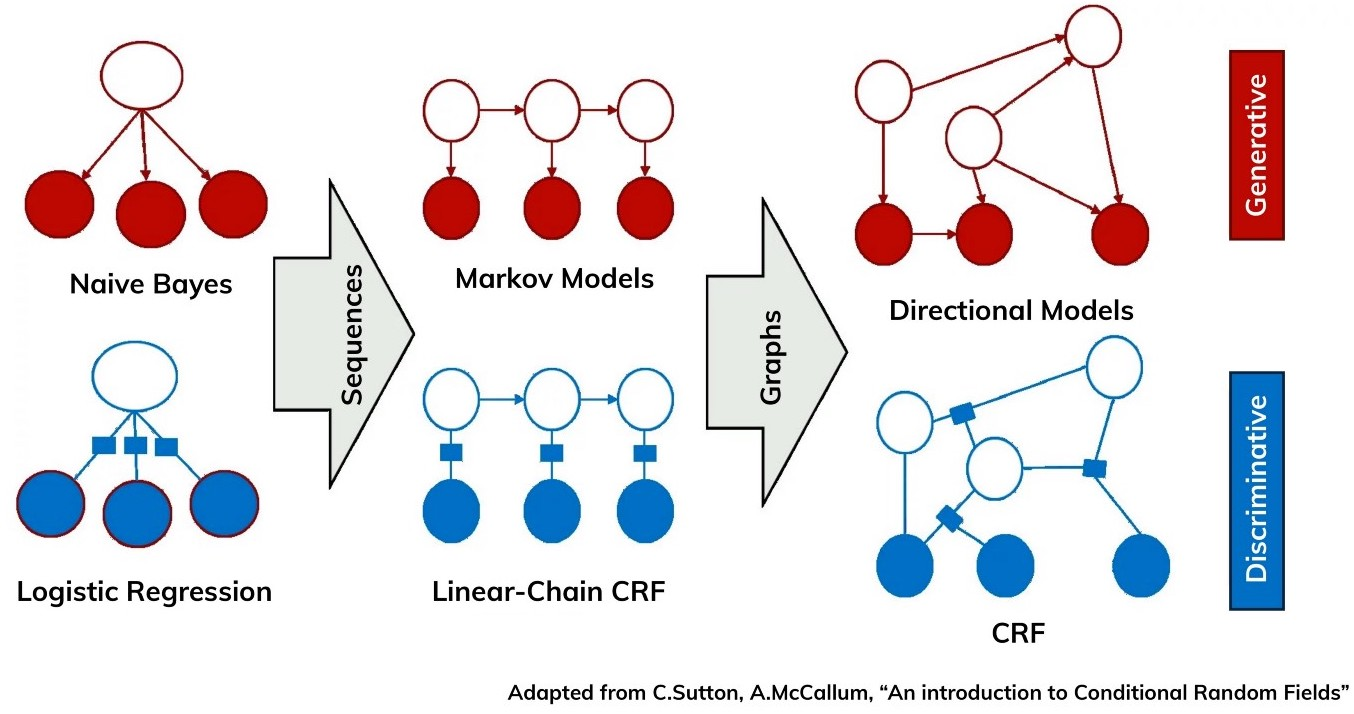
\includegraphics[width=14cm]{crf}
	\caption{Illustration presenting various families of graphical models. }
	\label{fig:graphical_models}
\end{figure} \\

\section{Network of exclusive coincidence classes}

Figure \ref{fig:ecc_graphical_models} presents an example of  ECC. 
\begin{figure}[!htbp]
	\centering
	
	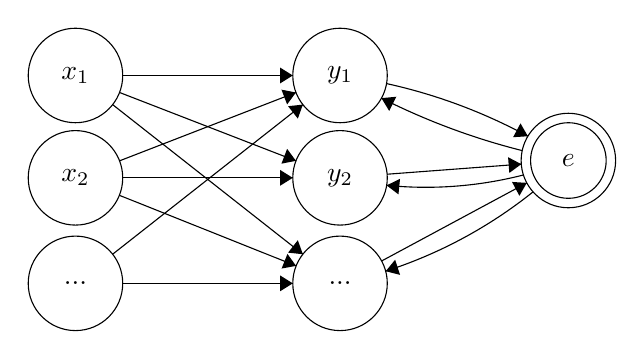
\begin{tikzpicture}[scale=0.2]
		\tikzstyle{every node}+=[inner sep=0pt]
		\draw [black] (40.1,-42.4) circle (3);
		\draw (40.1,-42.4) node {$e$};
		\draw [black] (40.1,-42.4) circle (2.4);
		\draw [black] (25.6,-37) circle (3);
		\draw (25.6,-37) node {$y_1$};
		\draw [black] (25.6,-43.5) circle (3);
		\draw (25.6,-43.5) node {$y_2$};
		\draw [black] (25.6,-50.2) circle (3);
		\draw (25.6,-50.2) node {$...$};
		\draw [black] (8.8,-37) circle (3);
		\draw (8.8,-37) node {$x_1$};
		\draw [black] (8.8,-43.5) circle (3);
		\draw (8.8,-43.5) node {$x_2$};
		\draw [black] (8.8,-50.2) circle (3);
		\draw (8.8,-50.2) node {$...$};
		\draw [black] (37.168,-41.77) arc (-104.11092:-116.74113:43.351);
		\fill [black] (28.23,-38.44) -- (28.72,-39.25) -- (29.17,-38.35);
		\draw [black] (37.246,-43.318) arc (-75.60821:-95.71526:24.95);
		\fill [black] (28.56,-43.98) -- (29.31,-44.55) -- (29.41,-43.56);
		\draw [black] (37.857,-44.391) arc (-51.32615:-72.11948:29.448);
		\fill [black] (28.5,-49.43) -- (29.41,-49.66) -- (29.1,-48.7);
		\draw [black] (11.8,-37) -- (22.6,-37);
		\fill [black] (22.6,-37) -- (21.8,-36.5) -- (21.8,-37.5);
		\draw [black] (11.6,-42.42) -- (22.8,-38.08);
		\fill [black] (22.8,-38.08) -- (21.88,-37.9) -- (22.24,-38.84);
		\draw [black] (11.16,-48.35) -- (23.24,-38.85);
		\fill [black] (23.24,-38.85) -- (22.3,-38.95) -- (22.92,-39.74);
		\draw [black] (11.6,-38.08) -- (22.8,-42.42);
		\fill [black] (22.8,-42.42) -- (22.24,-41.66) -- (21.88,-42.6);
		\draw [black] (11.16,-38.85) -- (23.24,-48.35);
		\fill [black] (23.24,-48.35) -- (22.92,-47.46) -- (22.3,-48.25);
		\draw [black] (11.8,-43.5) -- (22.6,-43.5);
		\fill [black] (22.6,-43.5) -- (21.8,-43) -- (21.8,-44);
		\draw [black] (11.8,-50.2) -- (22.6,-50.2);
		\fill [black] (22.6,-50.2) -- (21.8,-49.7) -- (21.8,-50.7);
		\draw [black] (11.59,-44.61) -- (22.81,-49.09);
		\fill [black] (22.81,-49.09) -- (22.26,-48.33) -- (21.89,-49.26);
		\draw [black] (28.555,-37.515) arc (77.60625:61.5417:34.266);
		\fill [black] (37.53,-40.86) -- (37.06,-40.04) -- (36.59,-40.92);
		\draw [black] (28.59,-43.27) -- (37.11,-42.63);
		\fill [black] (37.11,-42.63) -- (36.27,-42.19) -- (36.35,-43.19);
		\draw [black] (28.24,-48.78) -- (37.46,-43.82);
		\fill [black] (37.46,-43.82) -- (36.52,-43.76) -- (36.99,-44.64);
	\end{tikzpicture}
	\caption{An example of graphical model for exclusive coincidence classes. }
	\label{fig:ecc_graphical_models}
\end{figure}
The  $e$ node with double line represents an inhibitory neuron. All $y$ nodes are connected to it, meaning that they are mutually exclusive and only one of them can become active at the same time. All the excitatory $x$ nodes connected to any particular $y$ will contribute to its activation. The example above represents a bipartite graph, making it look like a feedforward network but in the more general case the directed connections could go both ways. The model does not need to be arranged in layers either.  

ECC are not trained using backpropagation. It is not even possible for two reasons. First is that binary values are not differentiable and second is that $\boldsymbol{y}$ are dependent on one another. Hebbian learning is necessary. 

Suppose that observation $\boldsymbol{x}$ produces certain vector of evidence $\boldsymbol{s}=\boldsymbol{x}W$. The winning explanation $y_k=1$ is then selected using $k=argmax_j s_j$. The remaining explanations are inactive $y_j=0$ for all other $j\ne k$.
The hebbian learning tells us to strengthen $w_{ji}$ for all $i$ such that $x_i$ is active. Neurons in ECC networks work like coincidence detectors and their goal is to build stronger connections with those inputs that often occur together. The update rule is as follows
\[
w_{ik} := w_{ik} + \epsilon \text{ if } x_i=1
\]
where $\epsilon$ is some small learning rate that defines plasticity of the neuron. Different neurons could potentially use distinct $\epsilon$ values. In the real brain this is often affected by neurotransmitters like dopamine. 

The hebbian rule above can only increment the weights. In order to prevent them from becoming too large, we follow this update by a normalization step.
\[
w_{ik} := \frac{w_{ik}}{ \sum_{ï} w_{ïk}} 
\]
The weights within a column must sum up to $1$. As a result, the connections $w_{ik}$ that rarely drive activity of $y_k$ will gradually vanish. There are several homeostatic processes in the biological neurons that could potentially implement such mechanism.  
It is possible that a single neuron might fire significantly more often than others. In order to make optimal use of all units, a form of entropy maximisation is necessary. We implement it using the vector $\boldsymbol{a}$. Each neuron $y_j$ has a corresponding activity value $a_j$.
When $y_j$ fires, we decrement $a_j$ by a constant factor.
\[
a_j := a_j - \alpha \text{ if } y_j \text{ fired}
\]
Now we can include $\boldsymbol{a}$ in the computation of $k$.
\[\boldsymbol{s} = \boldsymbol{x}W \]
\[\boldsymbol{r} = \boldsymbol{s} + \boldsymbol{a} \]
\[k = \argmax_j r_j \]
The final algorithm looks as follows
\begin{lstlisting}
def infer($\boldsymbol{x}$,$W$,$a$,learning_enabled):
    $s$ = $\boldsymbol{x}W$
    $r$ = $s + a$
    $k$ = argmax($r$)
    if $s_k$ $\le$ threshold:
        pass    // filter-out noise (optional)
    if learning_enabled:
        $a_k$ = $a_k$ - $\alpha$
        $W_k$ = $W_k+\boldsymbol{x}\epsilon$
        $W_k$ = $W_k$ / sum($W_k$)
        // the $W_k$ notation stands for 
        // k-th column of matrix $W$
    return $k$
\end{lstlisting}


\section{Fundamental theory}

\paragraph{ECC networks and Bayesian inference}  Learning the joint probability $p(\boldsymbol{x})$ is a daunting task. Belief nets, deep neural networks and graphical models attempt to factor out this distribution as
\[
p(\boldsymbol{x})=\prod_{y} p(\boldsymbol{y}|\pi(y))
\]
where $\pi(y)$ denotes parent/neighbours of $y$ in the graph. ECC networks take a different approach: 
\[
p(\boldsymbol{x})=\sum_{j} p(\boldsymbol{x},y_j)
\]
We could say that the two are ``orthogonal'' to each other in the sense that one is a multiplicative and the other is an additive factorization of $p(\boldsymbol{x})$.  While Bayesian and variational inference rely on independence of certain nodes $p(\boldsymbol{x})=p(x_1|\boldsymbol{y})p(x_2|\boldsymbol{y})...p(x_n|\boldsymbol{y})$, ECC try to partition $p(\boldsymbol{x})$ into mutually exclusive ``coincidence classes''
$p(\boldsymbol{x})=p(\boldsymbol{x},y_1)+p(\boldsymbol{x},y_2)+...+p(\boldsymbol{x},y_m)$. It could be seen as a linear combination of joint probability distributions
\[
p(\boldsymbol{x})=\sum_{j} p(\boldsymbol{x}|y_j) p(y_j)
\]
where $p(\boldsymbol{x}|y_j)$ are vectors and $p(y_j)$ are scalars with the constraint that all  $p(y_j)$ sum up to one $\sum_{j} p(y_j)=1$. The conditional probability $p(\boldsymbol{x}|y_j)$  may be difficult  to model directly. ECC network will build an approximate distribution $q(\boldsymbol{x}|y_j)$, which is easier to model. 
\[
p(\boldsymbol{x})\approx\sum_{j} q(\boldsymbol{x}|y_j) p(y_j)
\]
Such density function is parameterised using weight matrix $W$.
\paragraph{Interpretations of $W$ matrix}  It is possible to turn an ECC network ``upside-down'' and use it as a generative model.
\begin{lstlisting}
def generate(c, W, j):
    $\boldsymbol{x}$ = [0, 0, ... , 0] // n zeroes
    repeat c times:
        $i$ = random($W_j$)
        $x_i$ = 1
    return $\boldsymbol{x}$
\end{lstlisting}
The \texttt{random} function chooses a number between $1$ and $n$ according to distribution provided by $W_j$ ($j^{th}$ column of $W$). The \texttt{generate} function can be used to produce observation $\boldsymbol{x}$ with cardinality $\lVert\boldsymbol{x} \rVert_1$ (number of ones) less than or equal to $c$.  The probability of generating $\boldsymbol{x}$ in exactly $c=\lVert\boldsymbol{x} \rVert_1$ steps is given by 
 \[
 q(\boldsymbol{x}|y_j, \lVert\boldsymbol{x} \rVert_1 = c) = \frac{c!}{n^c}\prod_{x_i\in\boldsymbol{x}} w_{ij}
 \]
 The weights represent probability $w_{ij} = q(i| y_j)$, defined as
\begin{gather*}
\sum_{i=1}^{n} q(i | y_j) = 1 \\
q(i | y_j) =
\frac{\sum_{\boldsymbol{x}\in\{0,1\}^n}x_i  q(\boldsymbol{x}|y_j) }{\sum_{ï=1}^{n} \sum_{\boldsymbol{x}\in\{0,1\}^n}    x_{ï}  q(\boldsymbol{x}|y_j) } = \frac{\mathbb{E}_q(x_i|y_j)}{\sum_{ï=1}^{n} \mathbb{E}_q(x_{ï}|y_j)} =  \frac{q(x_i{=}1|y_j)}{\sum_{ï=1}^{n} q(x_{ï}{=}1|y_j)} 
\end{gather*}
In vector notation we obtain
\[
W_j = \frac{\mathbb{E}_q(\boldsymbol{x}|y_j)}{\lVert \mathbb{E}_q(\boldsymbol{x}|y_j) \rVert _1}\text{ where }\lVert \cdot \rVert _1\text{ is }\ell^1\text{ norm}
\]
Each column $W_j$ is a an expected value of binary vector, whose sum is normalised to $1$. The equality  $q(x_i{=}1|y_j)=\mathbb{E}_q(x_i|y_j)$ holds, because $x_i$ is a binary random variable. Analogically $q(x_i{=}0|y_j)=1-\mathbb{E}_q(x_i|y_j)$, hence $q(x_i|y_j)=|\mathbb{E}_q(x_i|y_j)-1+x_i|$.

 \paragraph{Models of $q(\boldsymbol{x}|y_j)$ distribution}
 The probability $q(\boldsymbol{x}|y_j)$ can be modelled as
 \begin{gather*} 
q(\boldsymbol{x}|y_j) = q(\boldsymbol{x}|y_j,c<\infty) = \sum_{c=0}^{\infty} p(c) q(\boldsymbol{x}|y_j,c)
 \end{gather*}
The term $q(\boldsymbol{x}|y_j,c)$ always has the following form
\[
q(\boldsymbol{x}|y_j,c) = N(\lVert\boldsymbol{x} \rVert_1 ,y_j,c)\big(\sum_{x_i\in\boldsymbol{x}} w_{ij}\big)^{ c - \lVert\boldsymbol{x} \rVert_1  }\prod_{x_i\in\boldsymbol{x}} w_{ij}
\]
where $N(\lVert\boldsymbol{x} \rVert_1 ,y_j,c)$ is some combinatorial coefficient that depends only on cardinality of $\boldsymbol{x}$ but not its contents. The inner product  $\boldsymbol{x}W_j$ gives us the probability of choosing any bit from $\boldsymbol{x}$
\[
\boldsymbol{x}W_j = \sum_{x_i\in\boldsymbol{x}} w_{ij}
\]
Let $\boldsymbol{x}', \boldsymbol{x}$ be two binary vectors, then $\boldsymbol{x}' \subset \boldsymbol{x}$ holds if $x_i'$ implies $x_i$. The probability of generating a subset of $\boldsymbol{x}$ is given by
\[
q(\boldsymbol{x}' \subset \boldsymbol{x}|y_j,c) = (\boldsymbol{x}W_j)^c
\]
Suppose that we run the generation process infinitely  $c=\infty$ with some probability $\beta$ of halting at any iteration. Then 
\begin{gather*}
q(\boldsymbol{x}' \subset \boldsymbol{x}|y_j,\beta) = \beta + (1-\beta)\boldsymbol{x}W_j q(\boldsymbol{x}' \subset \boldsymbol{x}|y_j,\beta) \\
q(\boldsymbol{x}' \subset \boldsymbol{x}|y_j,\beta)(1-(1-\beta)\boldsymbol{x}W_j ) = \beta \\
q(\boldsymbol{x}' \subset \boldsymbol{x}|y_j,\beta) = \frac{\beta}{1-(1-\beta)\boldsymbol{x}W_j } \\
\end{gather*}
\paragraph{Interpretations of  $\boldsymbol{x}W$ product}
Let $W_h,W_j \in \mathbb{R}^n$ be two weight vectors corresponding to $y_h$ and $y_j$. If $\boldsymbol{x}W_h \ge \boldsymbol{x}W_j$ then the following $2$ inequalities hold
\begin{gather*}
q(\boldsymbol{x}' \subset \boldsymbol{x} |y_h,\beta) \ge q(\boldsymbol{x}' \subset \boldsymbol{x} |y_j,\beta) \\
\lVert \boldsymbol{x} - W_h \rVert_1 \le \lVert  \boldsymbol{x} - W_j \rVert_1
\end{gather*}
The first inequality follows easily from its definition. The third one is proved below.
\begin{proof}
	\begin{gather*}
		\boldsymbol{x} W_h \ge \boldsymbol{x} W_j \\
		\sum_{x_i\in\boldsymbol{x} }w_{ih} \ge \sum_{x_i\in\boldsymbol{x} }w_{ij} \\
		\sum_{x_i\in\boldsymbol{x} }1-w_{ih} \le \sum_{x_i\in\boldsymbol{x} }1-w_{ij} \\
		\sum_{x_i\in\boldsymbol{x} }\vert 1-w_{ih}\vert \le \sum_{x_i\in\boldsymbol{x} }\vert 1-w_{ij}\vert
	\end{gather*}
	Let $1-\boldsymbol{x}$ be the complement of binary vector (ones and zeroes flipped). Because weights sum up to $1$, this implies that
	\begin{gather*}
		(1-\boldsymbol{x}) W_h \le (1-\boldsymbol{x}) W_j \\
		\sum_{x_i\notin\boldsymbol{x} }w_{ih} \le \sum_{x_i\notin\boldsymbol{x} }w_{ij} \\
		\sum_{x_i\notin\boldsymbol{x} }\vert 0-w_{ih}\vert \le \sum_{x_i\notin\boldsymbol{x} }\vert 0-w_{ij}\vert
	\end{gather*}
	Adding the two inequalities together by sides we obtain
	\[
	\lVert \boldsymbol{x} - W_h \rVert_1 \le \lVert  \boldsymbol{x} - W_j \rVert_1
	\]
\end{proof}

\paragraph{Binary vector subsets and their overlap probabilities} 

The number of all sparse binary vectors $\boldsymbol{x}$ of length $n$ and cardinality $\lVert\boldsymbol{x}\rVert_1$ is
\[\binom{n}{\lVert\boldsymbol{x}\rVert_1}\]
The $\ell_1$ norm induces a metric $\lVert\boldsymbol{x}-\boldsymbol{x}'\rVert_1$ on sparse binary vectors that measures how many bits differ in $\boldsymbol{x}$ and $\boldsymbol{x}'$. The inner product $\langle\boldsymbol{x},\boldsymbol{x}'\rangle$ measures number of overlapping $1$ bits. 
Given a specific $\boldsymbol{x}$, the number of all possible vectors $\boldsymbol{x}'$ that overlap with it in exactly $b$ bits is 
\[
\Omega(b)=|\{x':\langle\boldsymbol{x},\boldsymbol{x}'\rangle=b\}|=\binom{\lVert\boldsymbol{x}\rVert_1}{b}\binom{n-\lVert\boldsymbol{x}\rVert_1}{\lVert\boldsymbol{x}'\rVert_1-b}
\]
Therefore the probability that randomly chosen $\boldsymbol{x}'$ overlaps with $\boldsymbol{x}$ in at least $b$ bits is
\[p(\langle\boldsymbol{x},\boldsymbol{x}'\rangle\ge b )=\frac{\sum_{\dot{b}=b}^{\lVert\boldsymbol{x}'\rVert_1}\Omega(\dot{b})}{\binom{n}{\lVert\boldsymbol{x}\rVert_1}}\]
The probability of random $\boldsymbol{x}'$ being a subset of $\boldsymbol{x}$ is
\[p(\boldsymbol{x}'\subset\boldsymbol{x})=\frac{2^{\lVert\boldsymbol{x}\rVert_1}}{\binom{n}{\lVert\boldsymbol{x}\rVert_1}}\]
Both of those probabilities decrease factorially quickly with length $n$. For very sparse vectors, the chance of accidental overlap is almost zero. This property can be used to build noise-tolerant networks and to implement pattern completion.




\paragraph{Bits $x_i$ are mutually independent random variables} The \texttt{generate} function makes a certain implicit assumption. In each iteration, the next bit $x_i$ is randomly selected independently of the previous bits. As a result, all the bits are assumed to be mutually independent. 
\[
q(\boldsymbol{x}|y_j) = \prod_{i=1}^{n} q(x_i|y_j) = \big(\prod_{x_i\in\boldsymbol{x}} \mathbb{E}_q(x_i|y_j) \big) \big(\prod_{x_i\notin\boldsymbol{x}} 1-\mathbb{E}_q(x_i|y_j) \big)
\]
The expectation $\mathbb{E}_q(x_i|y_j) $ can be obtained from $W_j$ 
\begin{gather*}
\lVert \mathbb{E}_q(\boldsymbol{x}|y_j) \rVert _1 W_j = \mathbb{E}_q(\boldsymbol{x}|y_j) \\
\mathbb{E}_q(\lVert  \boldsymbol{x} \rVert _1|y_j)  W_j = \mathbb{E}_q(\boldsymbol{x}|y_j) 
\end{gather*}
If we know the expected cardinality of $\boldsymbol{x}$ in advance, then we can use the following function
\begin{lstlisting}
def generate2(c, W, j):
    $\boldsymbol{x}$ = [0, 0, ... , 0] // n zeroes
    for i from 1 to n:
        $p$ = $cw_{ij}$
        $x_i$ = random([$1-p$, $p$]) - 1
    return $\boldsymbol{x}$
\end{lstlisting}
The parameter $c$ is no longer used as a number of iterations, but as the expected cardinality $\mathbb{E}_q(\lVert  \boldsymbol{x} \rVert _1|y_j)$ instead. If we know the exact $\lVert  \boldsymbol{x} \rVert _1$ in advance, then it could be treated as a constant and the expected value becomes 
\begin{gather*}
\mathbb{E}_q(\lVert  \boldsymbol{x} \rVert _1|y_j)= \lVert  \boldsymbol{x} \rVert _1 = c \\
c w_{ij} = \mathbb{E}_q(x_i|y_j) = q(x_i{=}1|y_j)
\end{gather*}
\paragraph{Maximum likelihood estimation of W}
The $q(\boldsymbol{x}|y_j)$ distribution might be different from the true  $p(\boldsymbol{x}|y_j)$. Often we do not have access to $p(\boldsymbol{x})$ but we can use it to draw samples $X=[\boldsymbol{x}_1,\boldsymbol{x}_2,...]$  and then estimate an empirical distribution 
\[\bar{p}(\boldsymbol{x})=\frac{\text{ \# times }\boldsymbol{x}\text{ occurs in }X}{\text{ total \# of samples in}X}
\] 
This allows for inferring the optimal weights $W^*$ using maximum-likelihood estimation. 
\[
W_j^* = \argmax_{W_j}q(X|y_j;W_j)
\]
Because individual bits $q(x_i|y_j)$ are independent, we can efficiently infer the optimal $W_j$ for $q(\boldsymbol{x}|y_j)$, by inferring each $w_{ij}$ for $q(x_i|y_j)$ separately. 
\[
w_{ij}^* = \argmax_{w_{ij}}q(X|y_j;w_{ij}) = \frac{\mathbb{E}_X(x_i|y_j)}{c}
\]
\paragraph{Similarities between ECC and SVD}

The distribution $q(\boldsymbol{x})$ is modelled as a sum
\[
q(\boldsymbol{x}) = \sum_{j=1}^{m}q(\boldsymbol{x}|y_j)p(y_j)  = \sum_{j=1}^{m}\big(\prod_{i=1}^n q(x_i|y_j)\big)p(y_j) 
\]
Such factorization is motivated by the assumption that the external world has many latent causes $y_j$, and every one of them produces noisy observations $x_i$. The real world could potentially be approximated using trillions of latent causes, each one corresponding to some state of the world and objects in it. 

Many of the latent causes will produce similar or nearly identical observations. Could we exploit those similarities and compress our model (so that $m$ is as small as possible)? 

One way to reduce the number of $y$'s is by adding two (or more) of them as follows
\[
q(\boldsymbol{x}|y_1) p(y_1)+q(\boldsymbol{x}|y_2) p(y_2) = 
q(\boldsymbol{x}|y_1\text{ or }y_2) (p(y_1)+p(y_2))
\]
but storing $q(\boldsymbol{x}|y_1\text{ or }y_2)$ directly is impossible, because $W$ can only be used to represent mutually independent bits $x_i$. 
\begin{gather*}
q(x_i|y_1) p(y_1)+q(x_i|y_2) p(y_2) = c(w_{i1}p(y_1) +w_{i2}p(y_2))  \\
q(\boldsymbol{x}|y_1) p(y_1)+q(\boldsymbol{x}|y_2) p(y_2) \ne c(W_1p(y_1) +W_2p(y_2)) 
\end{gather*}
\underline{Hypothesis:} Perhaps there might be some way to reformulate certain aspects of linear algebra in a space of probability distributions 
\[p(\boldsymbol{x})\in \mathbb{R}^{2^n} \text{ such that } \lVert p(\boldsymbol{x}) \rVert_1=1\]
The task of reducing $m$ has certain similarities to matrix compression by performing SVD and truncating least significant eigenvalues. The receptive fields $p(\boldsymbol{x}|y_j)$ learned by neurons could be thought of as ``eigendistributions'' because they play analogical role to eigenvectors, i.e. every $p(\boldsymbol{x})$ is (approximately) a linear combination of eigendistributions $p(\boldsymbol{x}|y_j)$. The equality 
\[
\frac{q(\boldsymbol{x}|y_1;W_1) p(y_1)+q(\boldsymbol{x}|y_2;W_2) p(y_2)}{p(y_1)+p(y_2)} = 
q\big(\boldsymbol{x}|y_1\text{ or }y_2;\frac{W_1p(y_1) +W_2p(y_2)}{p(y_1)+p(y_2)}\big) 
\]
would hold only when $p(\boldsymbol{x},y_1)$ and $p(\boldsymbol{x},y_2)$ are colinear. If they are only approximately colinear, then the sum of $W_1$ and $W_2$ should still produce good approximation to $q(\boldsymbol{x}|y_1\text{ or }y_2)$. It looks like SVD, except that instead of truncating least significant eigenvalues, we cluster eigenvectors together by their similarity and then average them, producing $\mathbb{E}(\boldsymbol{x}|y_1\text{ or }y_2)$. The clustering algorithm implemented by ECC has some similarities to k-means.

\paragraph{Similarities between ECC and k-means }
The original \texttt{infer} algorithm implemented a form of online learning. Now let us suppose that we have some set of samples and we know the empirical distribution $\bar{p}(\boldsymbol{x})$. Define $C(y_j)$ as the cluster of all the $\boldsymbol{x}$ most similar to $W_j$ 
\[
C(y_j) = \{\boldsymbol{x} :  j = \argmax(\boldsymbol{x} W) \} 
\]
The mean $\mu(y_j)$ of cluster is given by 
\begin{gather*}
	\mathbb{E}_{\bar{p}}(\boldsymbol{x}|y_j) = \frac{\sum_{\boldsymbol{x}\in C(y_j)} \boldsymbol{x}\bar{p}(\boldsymbol{x})}{\sum_{\boldsymbol{x}\in C(y_j)} \bar{p}(\boldsymbol{x})} = \frac{\sum_{\boldsymbol{x}\in C(y_j)} \boldsymbol{x}\bar{p}(\boldsymbol{x})}{\bar{p}(y_j)} = \sum_{\boldsymbol{x}\in C(y_j)} \boldsymbol{x}\bar{p}(\boldsymbol{x}|y_j)\\
	\mu(y_j)  = \frac{\mathbb{E}_{\bar{p}}(\boldsymbol{x}|y_j)}{\sum_{ï=1}^{n}\mathbb{E}_{\bar{p}}(x_{ï}|y_j)}  = \frac{\mathbb{E}_{\bar{p}}(\boldsymbol{x}|y_j)}{\lVert \mathbb{E}_{\bar{p} }(\boldsymbol{x}|y_j)\rVert_1}
\end{gather*}
K-means clustering works by iteratively recomputing $C(y_j)^{(t)}$ at time-step $t$ for all $j$ and then assigning $\mu(y_j)^{(t)}$ to be the new value of $W_j^{(t+1)}$ at the next time-step. We in particular consider a generalisation of the k-means algorithm that uses learning rate $\epsilon$.
\begin{gather*}
W_j^{(t+1)} = (1-\epsilon)W_j^{(t)}+\epsilon \mu(y_j)^{(t)} 
\end{gather*} 
The difference between k-means and \texttt{infer} is the same as that between online and batch gradient-descent. Figures \ref{fig:k_means} presents results of learning with k-means. No entropy maximisation was used ($\alpha=0$).

\begin{figure}[!htbp]
	\centering
	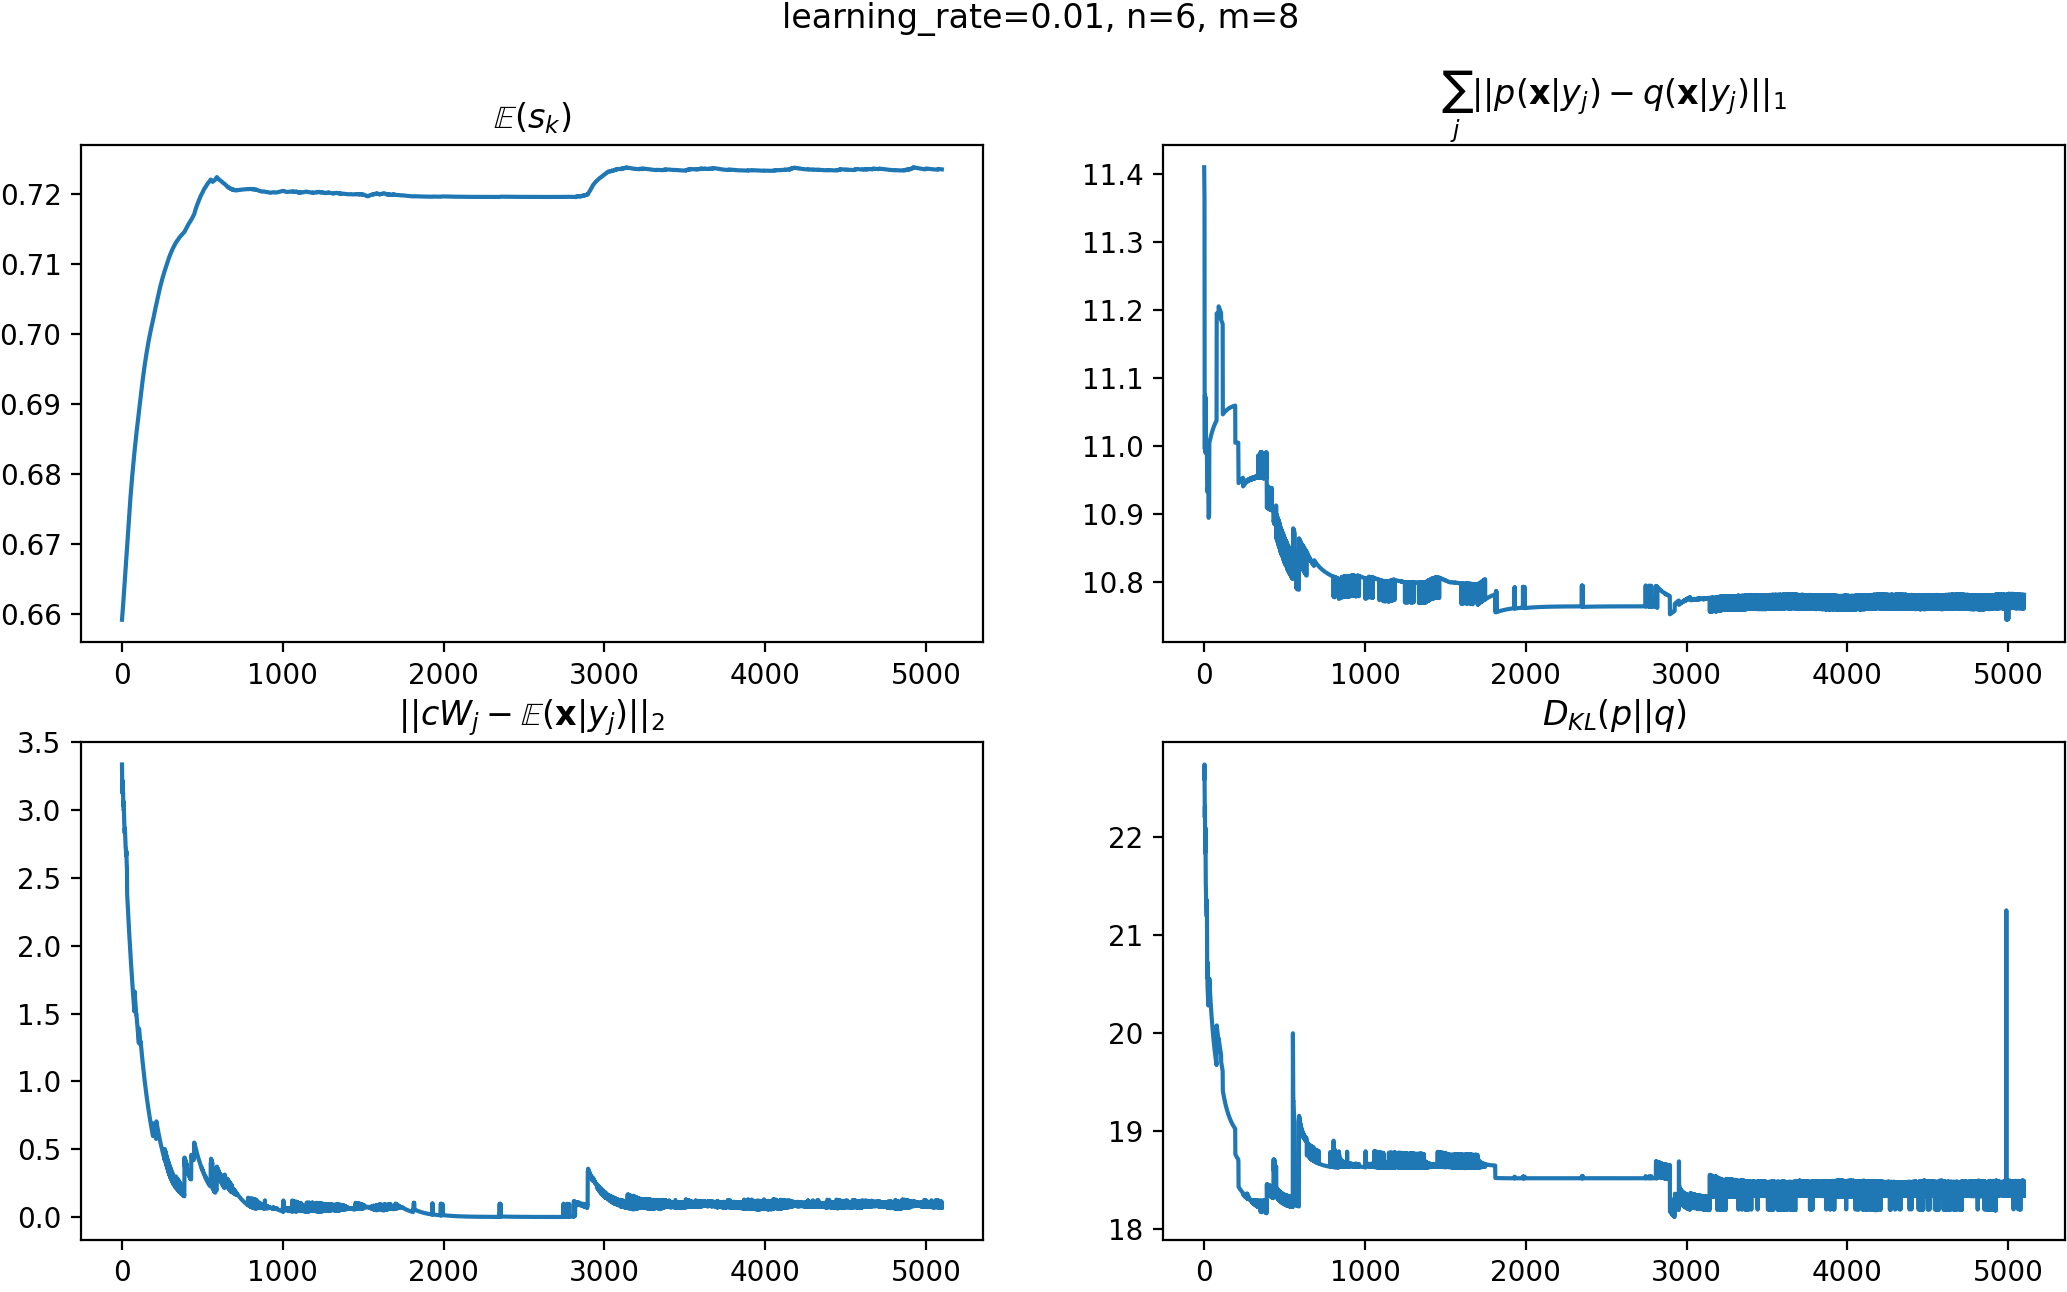
\includegraphics[width=13.5cm]{k_means_convergence}
	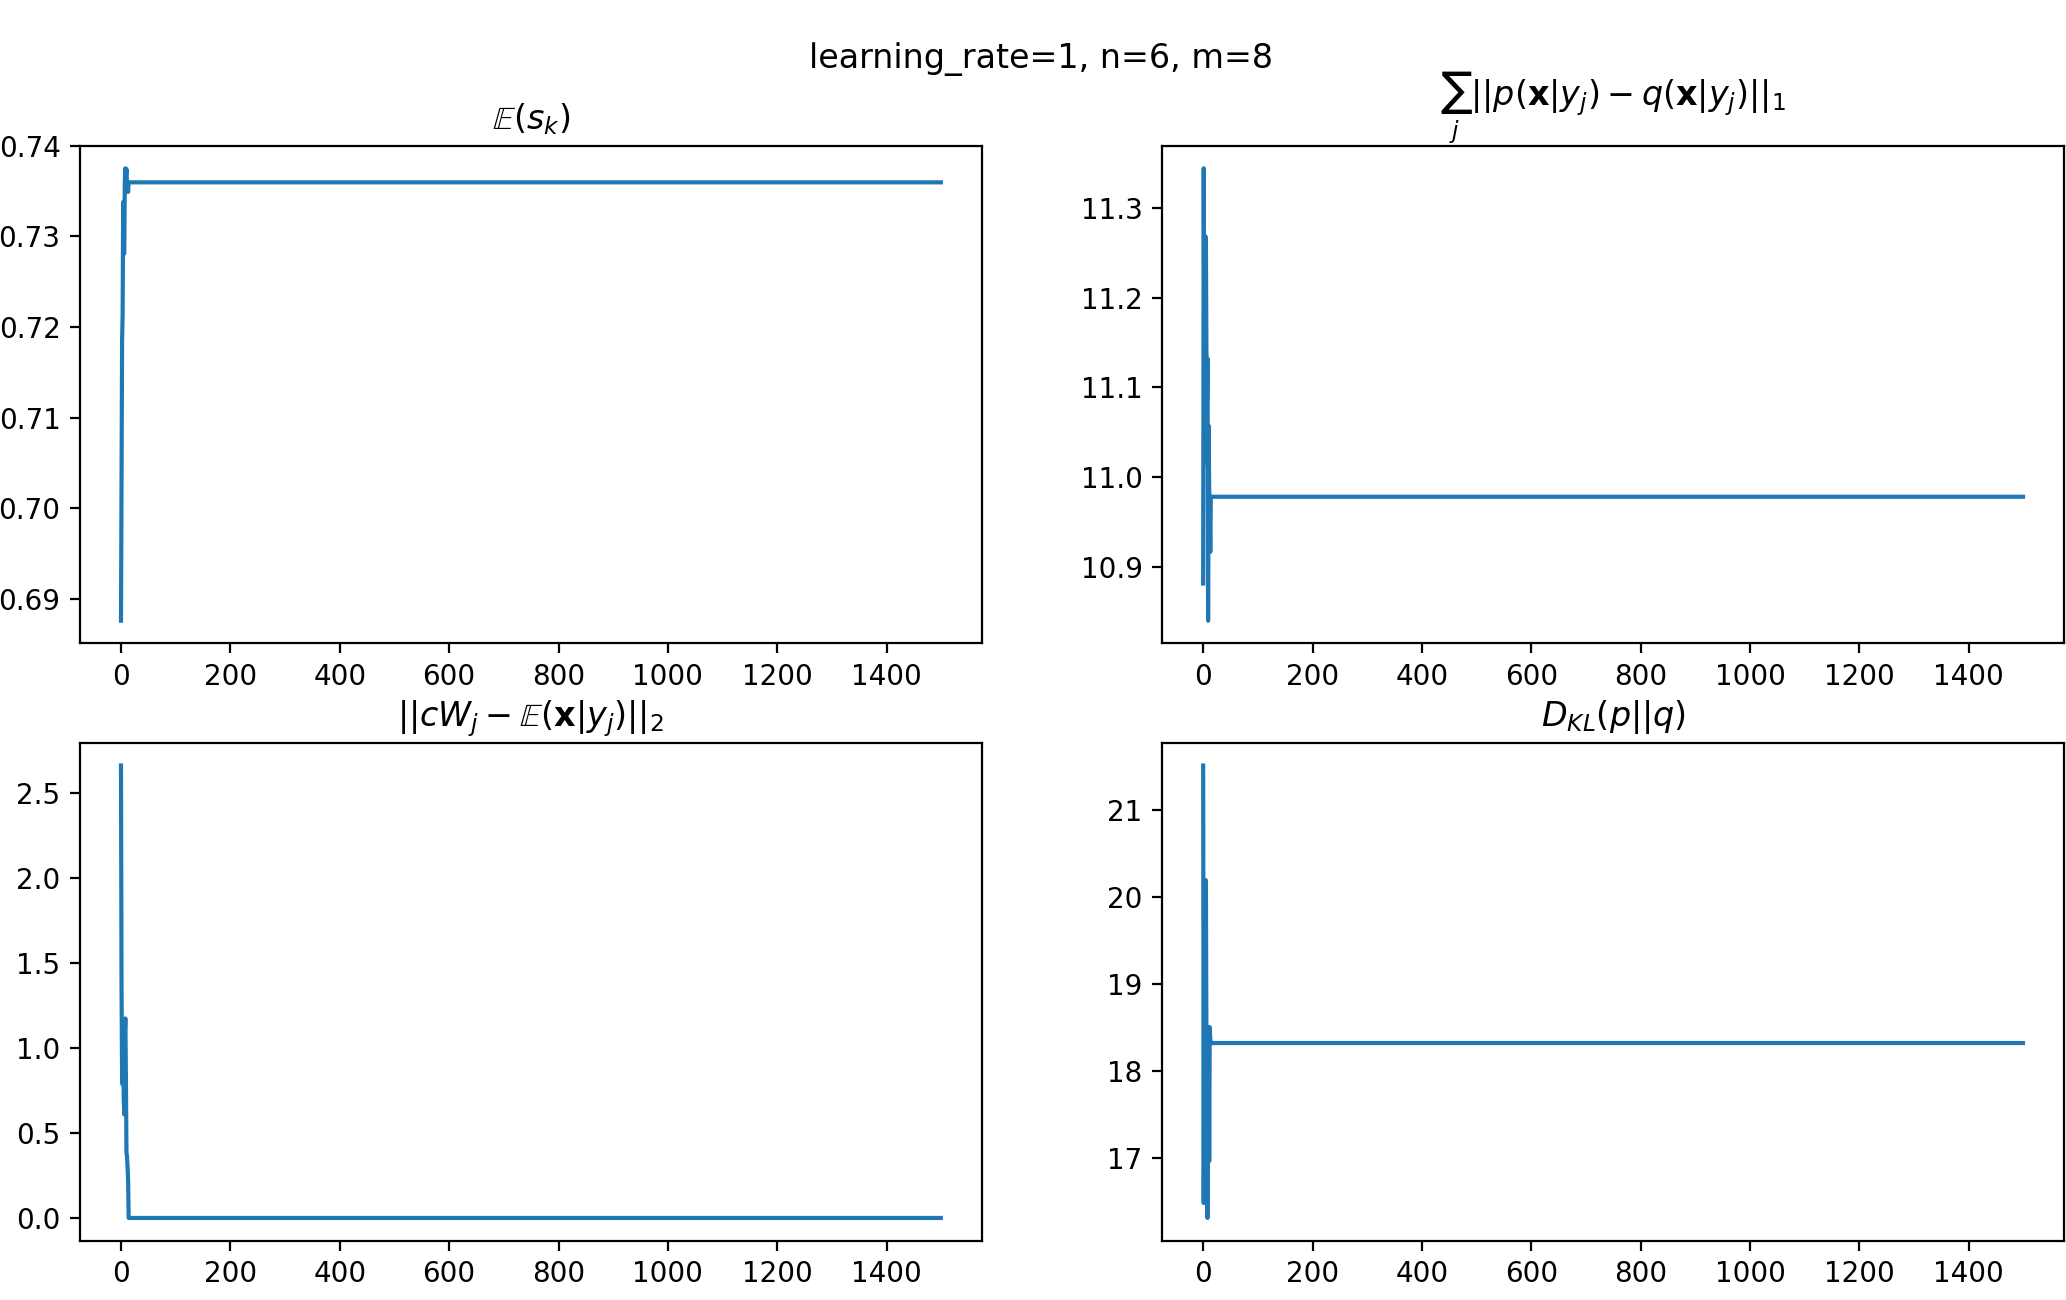
\includegraphics[width=13.5cm]{k_means_convergence2}
	\caption{Results of learning on randomly generated data $\bar{p}$ with $\epsilon=0.01$ (top) and $\epsilon=1$ (bottom). The horizontal axis in all graphs refers to time-step $t$. $\mathbb{E}(s_k)$ shows that match $s_k=\boldsymbol{x}W_k$ gets better over time. $\lVert c W_j - \mathbb{E}(\boldsymbol{x}|y_j)\rVert_2$ shows that $W_j$ converges to $\mu(y_j)$. $D_{KL}$ is Kullback-Leibler divergence between $\bar{p}$ and $q$.}
	\label{fig:k_means}
\end{figure} 

\paragraph{\texttt{infer} and \texttt{generate} define two different models of $q(\boldsymbol{x})$}
We will now consider two models $q_g$ and $q_i$, first one according to \texttt{generate} and other defined by \texttt{infer}. The probability $q_g$ is modelled as before
\[
q_g(\boldsymbol{x}) = \sum_{j=1}^{m} q(\boldsymbol{x}|y_j)p(y_j)
\]
We know that \texttt{infer} function will assign each $\boldsymbol{x}$ only to its respective cluster $C(y_j)$. As a result the true joint probability (not the one modelled by \texttt{generate}) is
\[
q_i(\boldsymbol{x},y_j) = 0 \text{ when } \boldsymbol{x}\notin C(y_j)
\]
Therefore we can state $q_i$ as
\[
q_i(\boldsymbol{x}) = q(\boldsymbol{x}|y_k)p(y_k)\text{ where }\boldsymbol{x}\in C(y_k)
\]
Through learning, the two models should become approximately equal. In order to achieve such agreement, training  must increase $q(\boldsymbol{x}|y_k)$ and decrease all other $q(\boldsymbol{x}|y_j)$. 
\begin{gather*}
	q_g(\boldsymbol{x}) = 	\sum_{j=1}^{m} q(\boldsymbol{x}|y_j)p(y_j) \approx q(\boldsymbol{x}|y_k)p(y_k) = q_i(\boldsymbol{x}) \\
	\sum_{j\ne k} q(\boldsymbol{x}|y_j)p(y_j) \approx 0 
\end{gather*}
Any algorithm that maximizes $\sum_{\boldsymbol{x}\in C(y_k)}q(\boldsymbol{x}|y_k)$ will automatically minimise $\sum_{\boldsymbol{x}\notin C(y_k)} q(\boldsymbol{x}|y_k)$  because probabilities sum up to $1$. If $\sum_{\boldsymbol{x}\notin C(y_j)} q(\boldsymbol{x}|y_j)$ decreases across all $y_j$ and $p(y_j)$ stay constant then the following sum decreases
\[
	\sum_{j} \sum_{\boldsymbol{x}\notin C(y_j)} q(\boldsymbol{x}|y_j) p(y_j) = \sum_{\boldsymbol{x}} \sum_{j\ne k}  q(\boldsymbol{x}|y_j) p(y_j) \text{ where }\boldsymbol{x}\in C(y_k)
\]
Therefore it can be seen that maximization of $\sum_{\boldsymbol{x}\in C(y_k)}q(\boldsymbol{x}|y_k)$ will push $q_g$ closer to $q_i$.  The maximal possible value is $1$.  The probabilities of each individual $q(\boldsymbol{x}|y_k)$ should be proportional to empirically sampled distribution $\bar{p}(\boldsymbol{x}|y_k)$
\[
q(\boldsymbol{x}|y_k) \approx \bar{p}(\boldsymbol{x}|y_k) = \frac{\bar{p}(\boldsymbol{x})}{\sum_{\boldsymbol{x}\in C(y_k)}\bar{p}(\boldsymbol{x})}
\]


\paragraph{Proof of convergence for k-means algorithm}
The model $q_g$ will approximate $q_i$ through maximisation of $\sum_{\boldsymbol{x}\in C(y_k)}q(\boldsymbol{x}|y_k)$, but the conditional probabilities $q(\boldsymbol{x}|y_k)$ are parameterised with matrix $W$. This enforces mutual independence of bits. There might not exist any good way to maximise this sum in the general case. Therefore it's vital that all vectors within the same cluster $C(y_k)$ share lots of bits in common. 

Let us also recall that the probability of accidental overlap $p(\langle\boldsymbol{x},\boldsymbol{x}'\rangle\ge b )$ is very low for sparse vectors.
Clustering similar vectors together will enhance robustness of the model.



Subset probability $q(\boldsymbol{x}' \subset \boldsymbol{x} |y_h,\alpha)$  is a good approximation of $q(\boldsymbol{x} |y_h)$.  The \texttt{infer} function 
Let us define a loss function
\[
\mathcal{L} = q_i(\boldsymbol{x}|y_j)-q_g(\boldsymbol{x})
\] 
\[
   \mathcal{L} = \sum_{j=1}^{m} \sum_{\boldsymbol{x}\in C(y_j)} q_i(\boldsymbol{x}|y_j)-q_g(\boldsymbol{x})
\] 
\[\mathcal{L}(C(y_j)^{(t)},W^{(t)})\le \mathcal{L}(C(y_j)^{(t+1)},W^{(t+1)})\] 
If loss is also bounded from below then it must converge. The monotonicity could be proved in two steps. First show that  
\[\mathcal{L}(C(y_j)^{(t)},W^{(t)})\le \mathcal{L}(C(y_j)^{(t)},W^{(t+1)})\] 
and then  
\[\mathcal{L}(C(y_j)^{(t)},W^{(t+1)})\le \mathcal{L}(C(y_j)^{(t+1)},W^{(t+1)})\] 
I have already tried this with many different loss functions such as
\begin{gather*}
\mathcal{L} = \sum_{j=1}^{m} \sum_{\boldsymbol{x}\in C(y_j)} \lVert  W_j - \boldsymbol{x}\rVert_1 \bar{p}(\boldsymbol{x}) \\
\mathcal{L} = \sum_{j=1}^{m} \sum_{\boldsymbol{x}\in C(y_j)} \lVert  W_j - \boldsymbol{x}\rVert_2 \bar{p}(\boldsymbol{x}) \\
\mathcal{L} = -\sum_{j=1}^{m} \sum_{\boldsymbol{x}\in C(y_j)} \boldsymbol{x}W_j  \bar{p}(\boldsymbol{x}) \\
\mathcal{L} = \sum_{j=1}^{m} D_{KL}(\bar{p}(\boldsymbol{x}|y_j)||q(\boldsymbol{x}|y_j))\\
\mathcal{L} =  -\sum_{j=1}^{m} \sum_{\boldsymbol{x}\in C(y_j)} q(\boldsymbol{x}'\subset \boldsymbol{x}|y_j)
\end{gather*}
and other variations thereof, but no luck so far. Empirically it looks like something must be converging, though.

\section{Convolutional networks}

\paragraph{Convolutional topology and topological receptive fields} In  the general case the topology of an ECC network might be chaotic and highly recurrent. We distinguish a special subset of topologies that are arranged in a form of multi-layer convolutional networks. Figure \ref{fig:ecc_conv_machine} shows an example of a single convolutional layer. Several of them could be stacked to form a multi-layer network. 

\begin{figure}[!htbp]
	\centering
	
	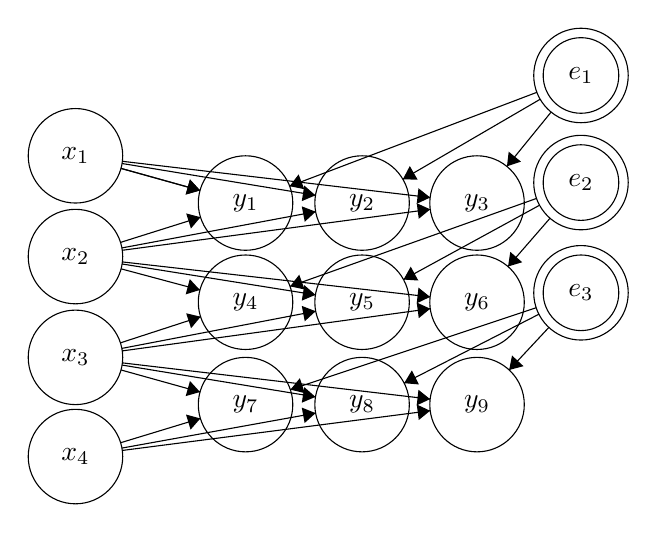
\begin{tikzpicture}[scale=0.2]
		\tikzstyle{every node}+=[inner sep=0pt]
		\draw [black] (8,-12.4) circle (3);
		\draw (8,-12.4) node {$x_1$};
		\draw [black] (8,-18.8) circle (3);
		\draw (8,-18.8) node {$x_2$};
		\draw [black] (8,-25.2) circle (3);
		\draw (8,-25.2) node {$x_3$};
		\draw [black] (8,-31.5) circle (3);
		\draw (8,-31.5) node {$x_4$};
		\draw [black] (18.8,-15.4) circle (3);
		\draw (18.8,-15.4) node {$y_1$};
		\draw [black] (33.5,-15.4) circle (3);
		\draw (33.5,-15.4) node {$y_3$};
		\draw [black] (26.2,-15.4) circle (3);
		\draw (26.2,-15.4) node {$y_2$};
		\draw [black] (18.8,-21.7) circle (3);
		\draw (18.8,-21.7) node {$y_4$};
		\draw [black] (26.2,-21.7) circle (3);
		\draw (26.2,-21.7) node {$y_5$};
		\draw [black] (33.5,-21.7) circle (3);
		\draw (33.5,-21.7) node {$y_6$};
		\draw [black] (18.8,-28.2) circle (3);
		\draw (18.8,-28.2) node {$y_7$};
		\draw [black] (26.2,-28.2) circle (3);
		\draw (26.2,-28.2) node {$y_8$};
		\draw [black] (33.5,-28.2) circle (3);
		\draw (33.5,-28.2) node {$y_9$};
		\draw [black] (40.1,-7.3) circle (3);
		\draw (40.1,-7.3) node {$e_1$};
		\draw [black] (40.1,-7.3) circle (2.4);
		\draw [black] (40.1,-14.1) circle (3);
		\draw (40.1,-14.1) node {$e_2$};
		\draw [black] (40.1,-14.1) circle (2.4);
		\draw [black] (40.1,-21.1) circle (3);
		\draw (40.1,-21.1) node {$e_3$};
		\draw [black] (40.1,-21.1) circle (2.4);
		\draw [black] (10.89,-13.2) -- (15.91,-14.6);
		\fill [black] (15.91,-14.6) -- (15.27,-13.9) -- (15,-14.86);
		\draw [black] (10.86,-17.9) -- (15.94,-16.3);
		\fill [black] (15.94,-16.3) -- (15.03,-16.06) -- (15.33,-17.02);
		\draw [black] (10.89,-13.2) -- (15.91,-14.6);
		\fill [black] (15.91,-14.6) -- (15.27,-13.9) -- (15,-14.86);
		\draw [black] (10.96,-12.89) -- (23.24,-14.91);
		\fill [black] (23.24,-14.91) -- (22.53,-14.29) -- (22.37,-15.28);
		\draw [black] (10.95,-18.25) -- (23.25,-15.95);
		\fill [black] (23.25,-15.95) -- (22.37,-15.61) -- (22.56,-16.59);
		\draw [black] (10.98,-12.75) -- (30.52,-15.05);
		\fill [black] (30.52,-15.05) -- (29.78,-14.46) -- (29.67,-15.45);
		\draw [black] (10.97,-18.4) -- (30.53,-15.8);
		\fill [black] (30.53,-15.8) -- (29.67,-15.41) -- (29.8,-16.4);
		\draw [black] (37.3,-8.37) -- (21.6,-14.33);
		\fill [black] (21.6,-14.33) -- (22.53,-14.52) -- (22.17,-13.58);
		\draw [black] (37.51,-8.81) -- (28.79,-13.89);
		\fill [black] (28.79,-13.89) -- (29.73,-13.92) -- (29.23,-13.05);
		\draw [black] (38.2,-9.63) -- (35.4,-13.07);
		\fill [black] (35.4,-13.07) -- (36.29,-12.77) -- (35.51,-12.14);
		\draw [black] (37.47,-15.54) -- (28.83,-20.26);
		\fill [black] (28.83,-20.26) -- (29.77,-20.32) -- (29.29,-19.44);
		\draw [black] (38.13,-16.37) -- (35.47,-19.43);
		\fill [black] (35.47,-19.43) -- (36.37,-19.16) -- (35.61,-18.5);
		\draw [black] (37.27,-15.11) -- (21.63,-20.69);
		\fill [black] (21.63,-20.69) -- (22.55,-20.89) -- (22.21,-19.95);
		\draw [black] (38.06,-23.3) -- (35.54,-26);
		\fill [black] (35.54,-26) -- (36.45,-25.76) -- (35.72,-25.08);
		\draw [black] (37.43,-22.46) -- (28.87,-26.84);
		\fill [black] (28.87,-26.84) -- (29.81,-26.92) -- (29.36,-26.03);
		\draw [black] (37.25,-22.05) -- (21.65,-27.25);
		\fill [black] (21.65,-27.25) -- (22.56,-27.47) -- (22.25,-26.52);
		\draw [black] (10.9,-19.58) -- (15.9,-20.92);
		\fill [black] (15.9,-20.92) -- (15.26,-20.23) -- (15,-21.2);
		\draw [black] (10.85,-24.28) -- (15.95,-22.62);
		\fill [black] (15.95,-22.62) -- (15.03,-22.4) -- (15.34,-23.35);
		\draw [black] (10.96,-19.27) -- (23.24,-21.23);
		\fill [black] (23.24,-21.23) -- (22.53,-20.61) -- (22.37,-21.6);
		\draw [black] (10.95,-24.63) -- (23.25,-22.27);
		\fill [black] (23.25,-22.27) -- (22.37,-21.93) -- (22.56,-22.91);
		\draw [black] (10.98,-19.14) -- (30.52,-21.36);
		\fill [black] (30.52,-21.36) -- (29.78,-20.77) -- (29.67,-21.77);
		\draw [black] (10.97,-24.79) -- (30.53,-22.11);
		\fill [black] (30.53,-22.11) -- (29.67,-21.72) -- (29.8,-22.71);
		\draw [black] (10.89,-26) -- (15.91,-27.4);
		\fill [black] (15.91,-27.4) -- (15.27,-26.7) -- (15,-27.66);
		\draw [black] (10.87,-30.62) -- (15.93,-29.08);
		\fill [black] (15.93,-29.08) -- (15.02,-28.83) -- (15.31,-29.79);
		\draw [black] (10.96,-25.69) -- (23.24,-27.71);
		\fill [black] (23.24,-27.71) -- (22.53,-27.09) -- (22.37,-28.08);
		\draw [black] (10.95,-30.96) -- (23.25,-28.74);
		\fill [black] (23.25,-28.74) -- (22.37,-28.39) -- (22.55,-29.37);
		\draw [black] (10.98,-25.55) -- (30.52,-27.85);
		\fill [black] (30.52,-27.85) -- (29.78,-27.26) -- (29.67,-28.25);
		\draw [black] (10.98,-31.11) -- (30.52,-28.59);
		\fill [black] (30.52,-28.59) -- (29.67,-28.19) -- (29.8,-29.18);
	\end{tikzpicture}
	\caption{A single layer of exclusive coincidence machine with one-dimensional convolution. The input size is $4$ columns, each with one channel. The hidden layer has $3$ columns, each with $3$ channels. The neurons within the same column are all mutually exclusive. Every hidden column draws input from two input columns around it, meaning that in this case the kernel size is $2$. The stride is $0$. }
	\label{fig:ecc_conv_machine}
\end{figure} 

The neuron $y_1$ can ``see'' input coming from $x_1$ and $x_2$. We say that the topological receptive field $\tau$ of $y_1$ is $\tau(y_1)=\{x_1,x_2\}$. All the neurons
within the same column share common $\tau$ and compete with each other due to inhibition. Neurons across different columns have access to distinct fragments of input. As a result every column will only learn to recognise input at a specific location. 

\paragraph{Translation invariance and column isomorphism}  Deep nets learn by approximating invariant/equivariant functions. In particular deep convolutional networks a-priori come with the assumption of translation equivariance, which is enforced by sharing kernel weights. The ECC are capable of learning such equivariances on their own, without sharing any weights.

In the example from figure \ref{fig:ecc_conv_machine}, the neurons $[y_1,y_2,y_3]$ and $[y_4,y_5,y_6]$ receive inputs $[x_1,x_2]$ and $[x_2,x_3]$ respectively. If the input is indeed translation invariant then $p([x_1,x_2])=p([x_2,x_3])$ should hold by definition. In such case, hebbian learning will drive both $[y_1,y_2,y_3]$ and $[y_4,y_5,y_6]$ to develop similar factorizations
\begin{gather*}
	p(\boldsymbol{x}) = p(\boldsymbol{x}|y_1)p(y_1)+  p(\boldsymbol{x}|y_2)p(y_2)+  p(\boldsymbol{x}|y_3)p(y_3)\text{ where }\boldsymbol{x}=[x_1,x_2] \\
	p(\boldsymbol{x}) = p(\boldsymbol{x}|y_4)p(y_4)+  p(\boldsymbol{x}|y_5)p(y_5)+  p(\boldsymbol{x}|y_6)p(y_6)\text{ where }\boldsymbol{x}=[x_2,x_3]
\end{gather*}
such that $p(\boldsymbol{x}|y_2) \approx p(\boldsymbol{x}|y_{\sigma(4)}), p(\boldsymbol{x}|y_{3}) \approx p(\boldsymbol{x}|y_{\sigma(5)}),p(\boldsymbol{x}|y_3) \approx p(\boldsymbol{x}|y_{\sigma(6)}) $ for some permutation $\sigma$. Both columns are approximately isomorphic. We can stack multiple layers on top of each other and the equivariance will be preserved. For example let $W_1,W_2$ be the weights of connections from $[y_1,y_2,y_3]$ and   $[y_4,y_5,y_6]$ respectively, outgoing to  neurons $z_1,z_c$ in next layer (with $c$ channels). If the two columns are isomorphic then $W_1\approx\sigma W_2$. Hence it can be seen that the networks can self-organise and equivariance will emerge. The only inductive bias is the topology $\tau$. (Convolutional pattern of $\tau$ can easily emerge on its own if we assume that the neurons are embedded in a physical space and the axons are sparsely projected to some small local neighbourhood in subsequent regions of neocortex.)

\paragraph{Multilayer networks}
ECC networks could be stacked on top of each other. By introducing another layer $\boldsymbol{z}$ we could approximate one $z_h$ using a combination of   $\boldsymbol{y}$
\[
q(\boldsymbol{x}|z_h) = \sum_{j} q(y_j|z_h) q(\boldsymbol{x}|y_j)
\] 
The probability $p(y_j|z_h)$ is not represented directly. The weights of connections between $\boldsymbol{y}$ and $\boldsymbol{z}$ only encode the probability $q(j|z_h)$, which is defined analogically as before. 

The \texttt{generate} function can be generalised to much deeper multi-layer architectures as follows
\begin{lstlisting}
// W_array contains W matrices of consecutive layers.
// The order is reverse (deepest layer comes first)
def generate_deep(c, W_array, j):
    $\boldsymbol{x}$ = [0, 0, ... , 0] // n zeroes
    repeat c times:
        i = j
        for $W$ in W_array
            i = random($W_i$)
        $x_i$ = 1
    return $\boldsymbol{x}$
\end{lstlisting}
This procedure will iteratively propagate the activation from top to bottom. It recursively models the following expectation
\[
\mathbb{E}(\boldsymbol{x}|z_j) = \sum_{i} p(i|z_j) \mathbb{E}(\boldsymbol{x}|y_i)
\] 
\paragraph{Probability $q(\boldsymbol{x})$ is relative} The \texttt{generate\_deep} procedure can be used to sample $\mathbb{E}(\boldsymbol{x}|z_j)$ but it does not yet define $q(\boldsymbol{x})$. Key observation is that the $j$ argument is still necessary and we have to decide which hidden neuron to sample. In order to define $q(\boldsymbol{x})$ for the network as a whole, some probability $p(z_j)$ is necessary. It could be modelled as $q(z_j|v_h)$ by some even deeper layers $\boldsymbol{v}$. This leads to a two-step generation process
\begin{lstlisting}
def generate_2step(c, W_to_choose_j, W_to_sample, h):
    j = argmax(generate_deep(1, W_to_choose_j, h))
    return generate_deep(c, W_to_sample, j)
\end{lstlisting}
The concatenation of arrays \texttt{W\_to\_choose\_j} and  \texttt{W\_to\_sample} could be seen as one large network. Universal approximation theorem can be proved using such a two-step generator
\paragraph{Training and its results}  Convolutional ECC networks can be trained either layer-by-layer (from bottom to top) or all at once (hebbian learning works everywhere simultaneously). The only difference between the two approaches is that training layer-by-layer can be much faster and more efficient on a static dataset, whereas online learning of all layers at once allows for extracting temporal dependencies in an interactive environment. 

Network topology is determined by its sequence of convolutions. Each layer is characterised by triple $(K, S, C)$ which stands for kernel $K \times K$, stride $S \times S$ and $C$ output channels. Here we present effects of all-at-once training for 3-layer architecture $(5,2,20) ,(2,1,49),  (3,1 ,64)$. Figures  \ref{fig:layer1},  \ref{fig:layer2} and  \ref{fig:layer3} show averaged receptive field $\mathbb{E}(\boldsymbol{x}|y_j)$ formed by one arbitrarily chosen column in the first, second and third hidden layer respectively.


\begin{figure}[!htbp]
	\centering
	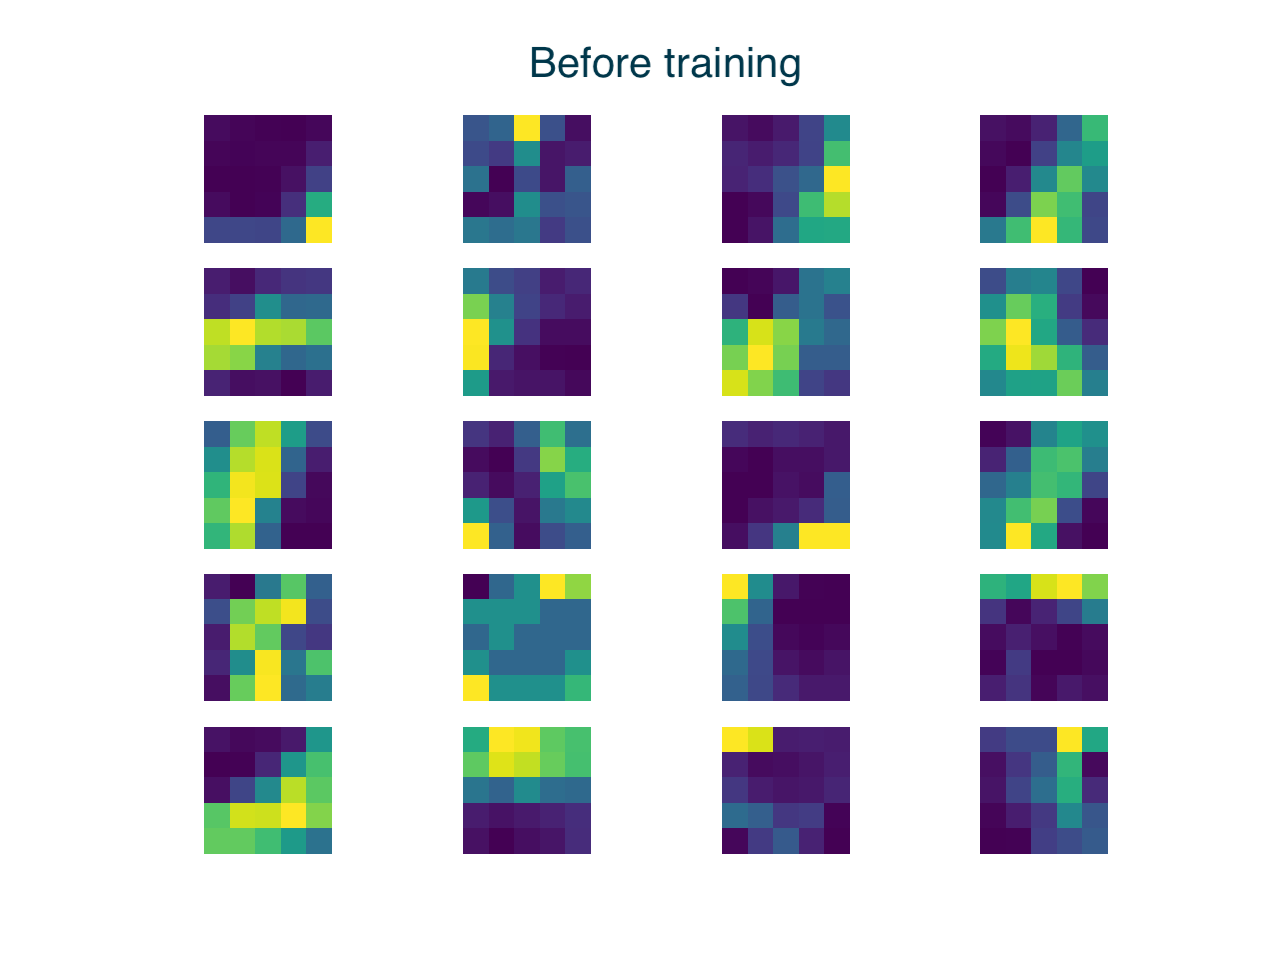
\includegraphics[width=12cm]{k5s2c1d1_c20 machine before}
	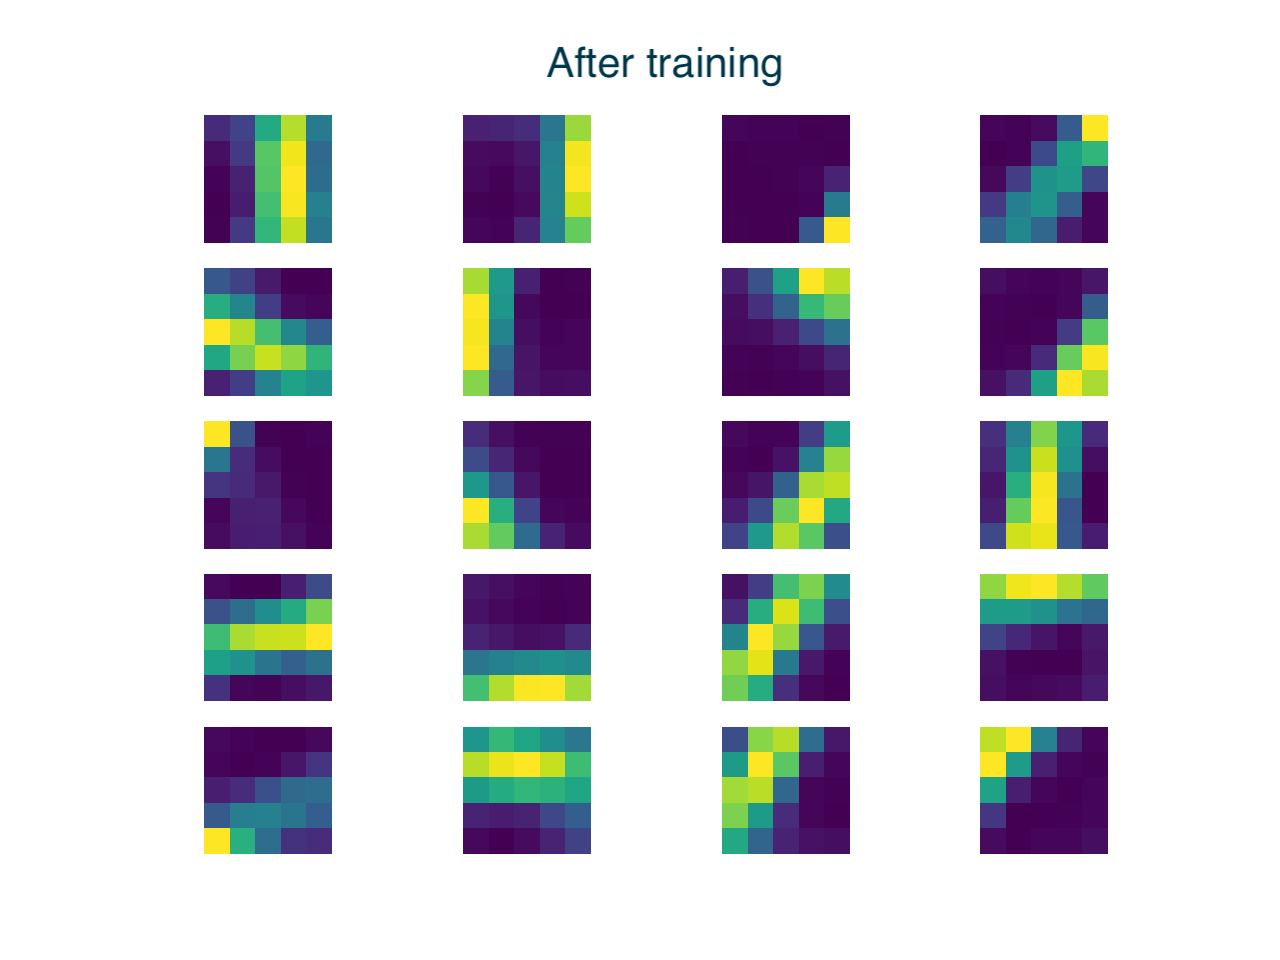
\includegraphics[width=12cm]{k5s2c1d1_c20 machine after}
	\caption{Receptive fields of 20 neurons from a column in the first hidden layer before and after training.}
	\label{fig:layer1}
\end{figure} 

\begin{figure}[!htbp]
	\centering
	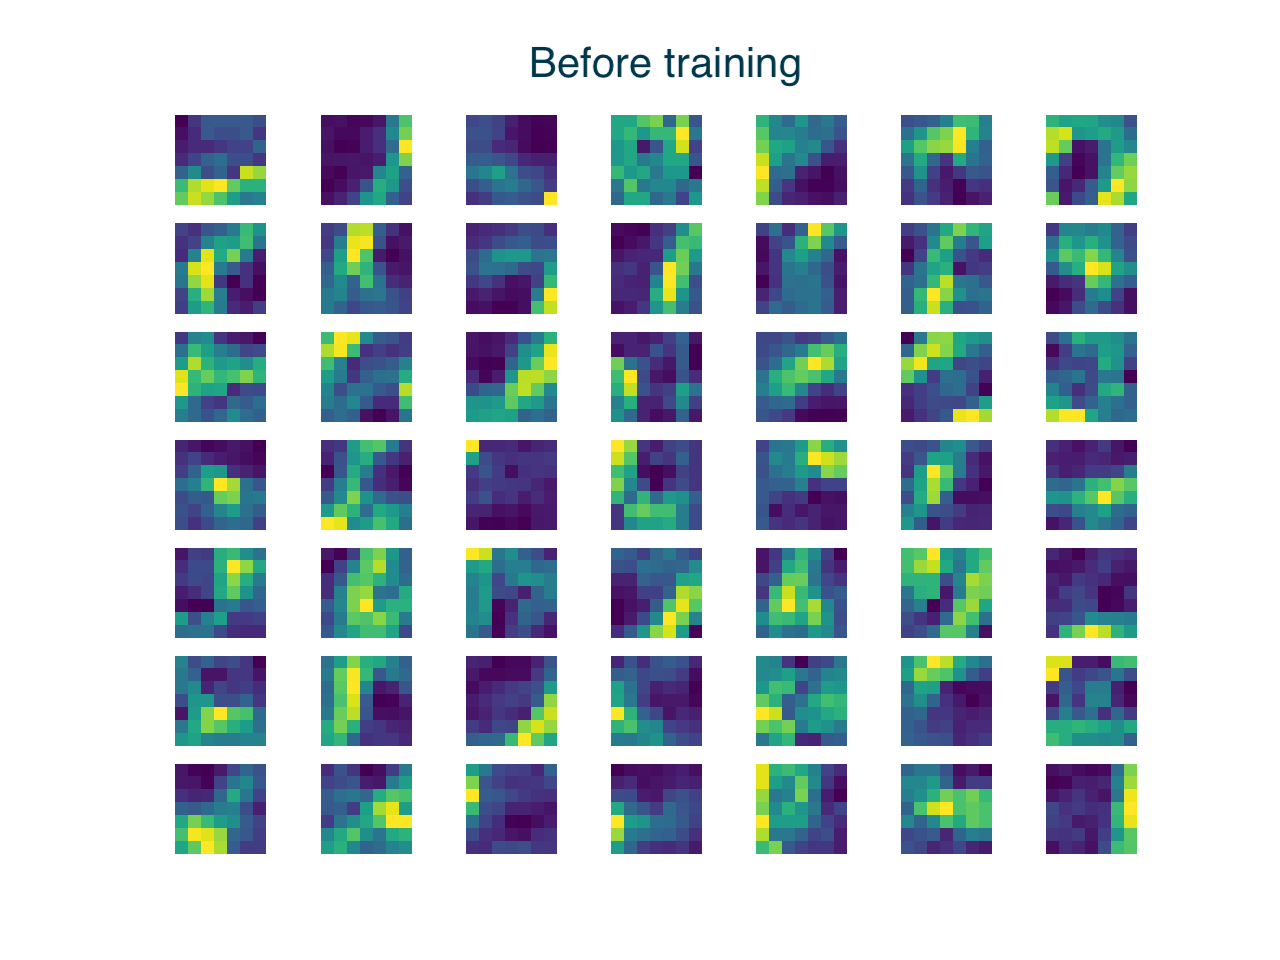
\includegraphics[width=11cm]{k5s2c1d1_k2s1c20d1_c49 machine before}
	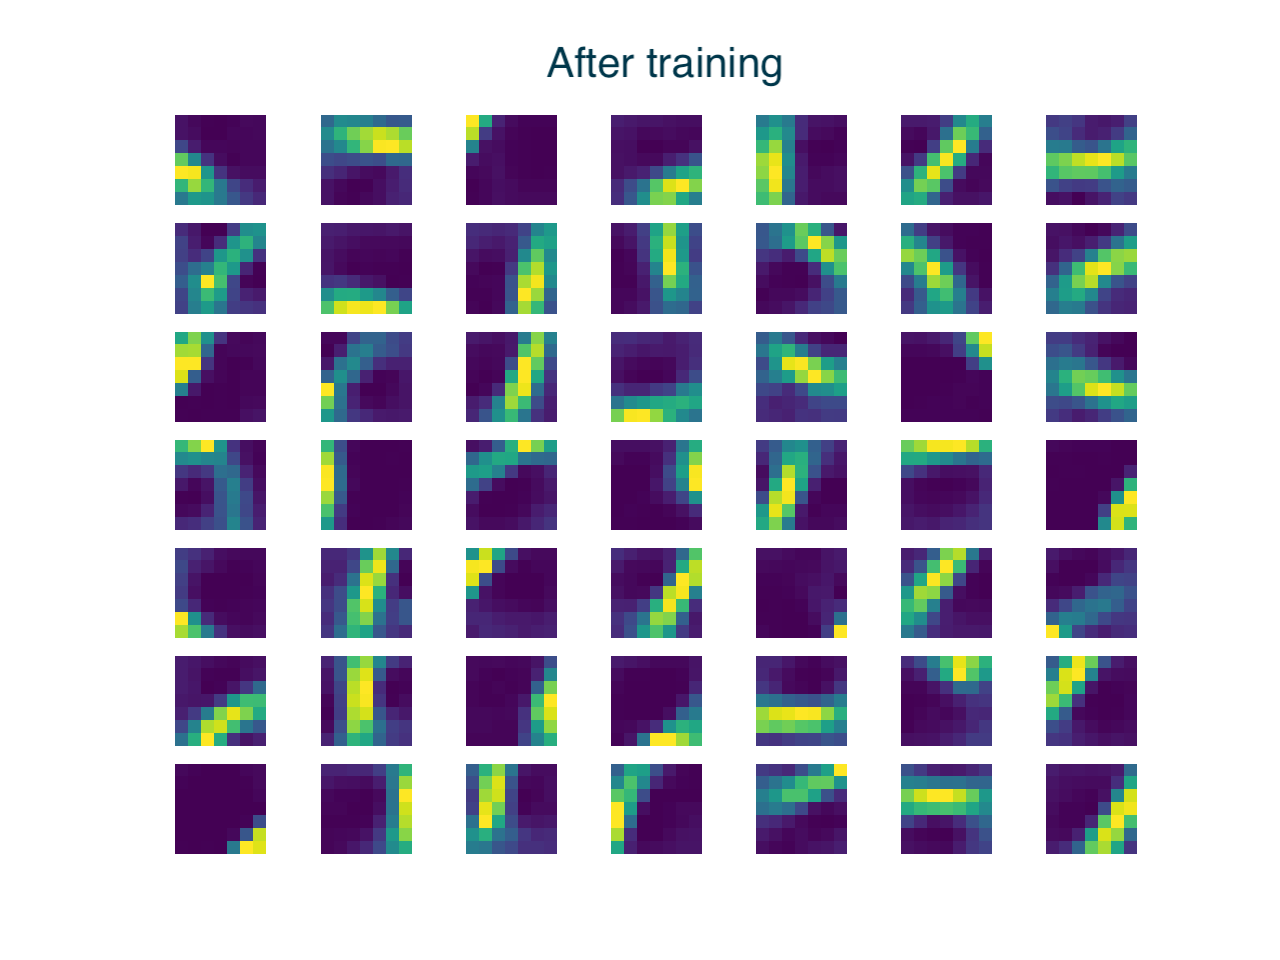
\includegraphics[width=11cm]{k5s2c1d1_k2s1c20d1_c49 machine after}
	\caption{Receptive fields of 49 neurons from a column in the second layer}
	\label{fig:layer2}
\end{figure} 

\begin{figure}[!htbp]
	\centering
	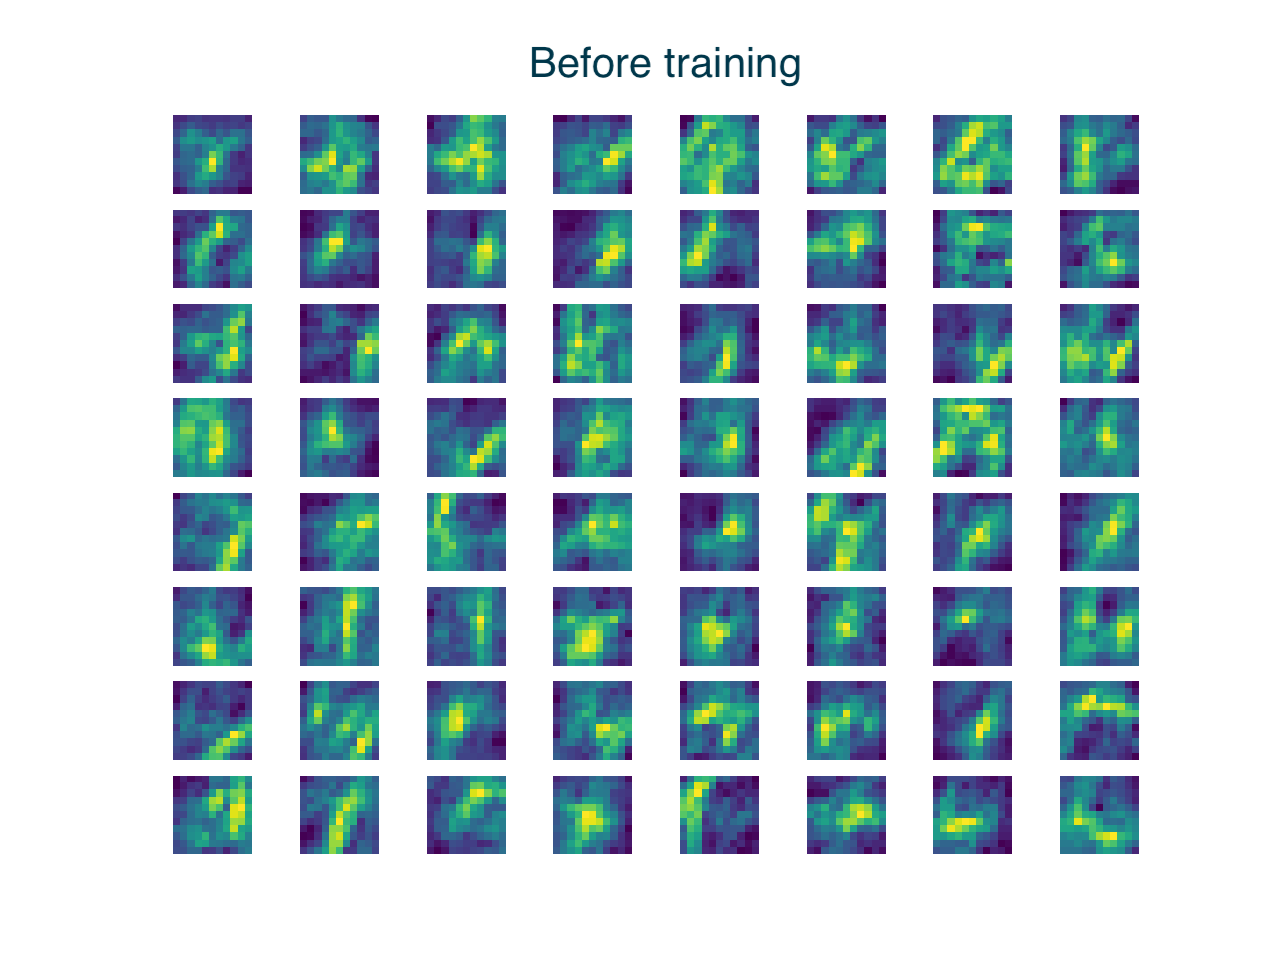
\includegraphics[width=11cm]{k5s2c1d1_k2s1c20d1_k3s1c49d1_c64 machine before}
	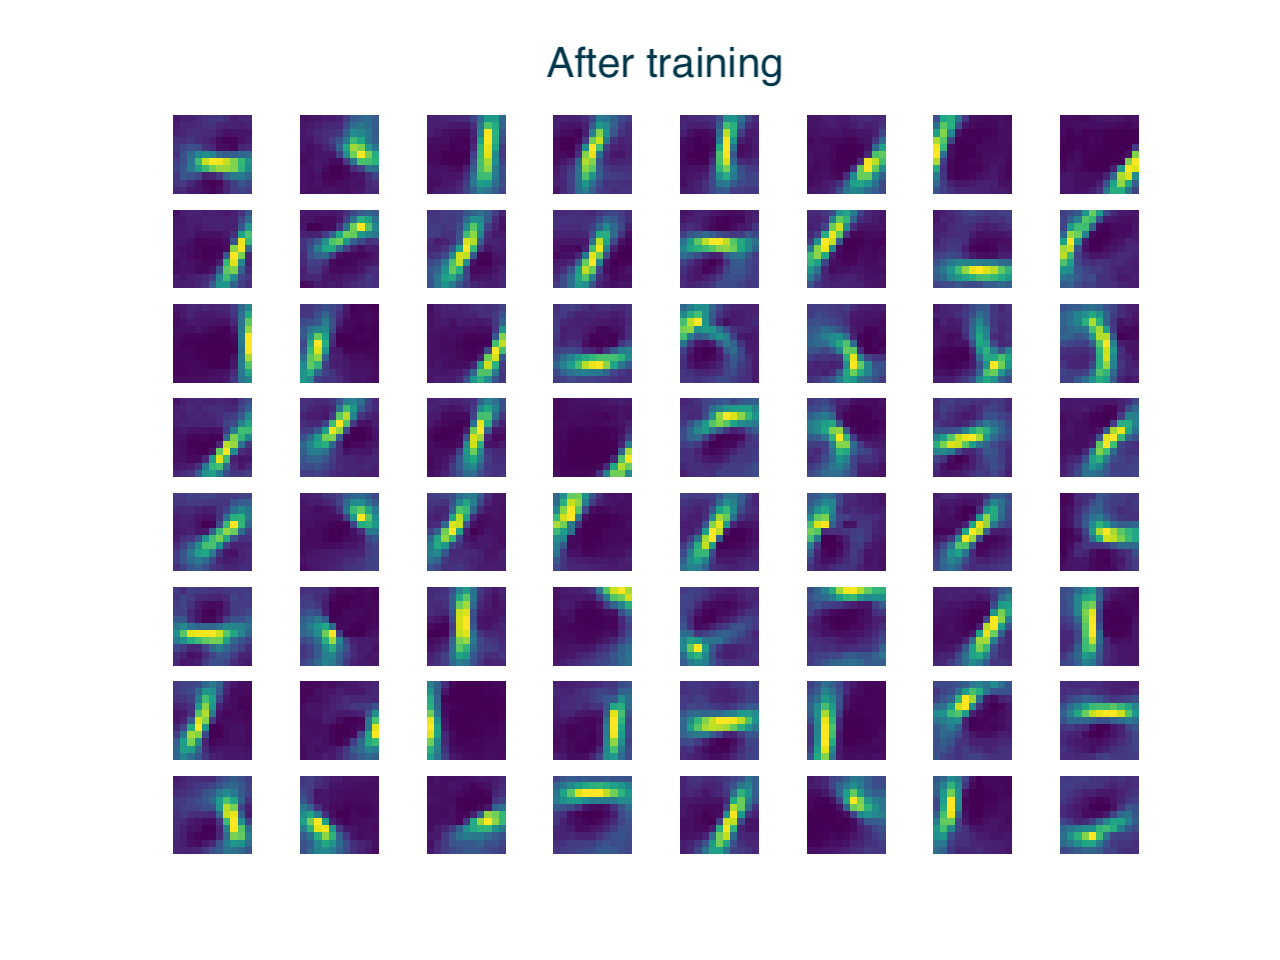
\includegraphics[width=11cm]{k5s2c1d1_k2s1c20d1_k3s1c49d1_c64 machine after}
	\caption{Receptive fields of 64 neurons from a column in the third layer}
	\label{fig:layer3}
\end{figure} 


\paragraph{Universal approximation}

ECC networks can approximate any $p(\boldsymbol{x})$ with only two layers. The first layer contains $2^n$ hidden neurons $\boldsymbol{y}$, one for every possible binary vector $\{0,1\}^n$. For every $\boldsymbol{x} \in \{0,1\}^n$, there exists $y_j$ such that the weights $W_j^{(\boldsymbol{y})}$ are uniformly distributed for all $x_i \in \boldsymbol{x}$ and zero everywhere else. The second layer $\boldsymbol{z}$ takes input from $\boldsymbol{y}$ and produces a single output $\boldsymbol{z}=[z_1]$. For every $y_j$ there exists a single weight $w_{j1}^{(\boldsymbol{z})}$ to $z_1$ whose value determines the probability $q(j|z_1)=p(y_j)$. 

The probability $p(\boldsymbol{x})$ will be correctly approximated if we can show that the ECC network generates samples using the same distribution. The \texttt{generate} function expects $j$ as one of its parameters. We can choose it using the second layer and then run \texttt{generate(c,W,j)} for some sufficiently large number $c=\infty$. This will almost surely result in producing  $\boldsymbol{x}$ such that $x_i\in \boldsymbol{x}$ for all $W_{ij}>0$. This entire procedure could be summarised as 
\begin{lstlisting}
generate_2step($\infty$, [$W^{(\boldsymbol{z})}$], [$W^{(\boldsymbol{y})}$], 1)
\end{lstlisting}

\paragraph{Problem with distinguishing bit subsets} The universal approximation holds, even though the constructed network has one significant flaw. For any two $\boldsymbol{x}'$, $\boldsymbol{x}$ such that one is a subvector of the other $\boldsymbol{x}'\subset \boldsymbol{x}$, the \texttt{infer} function will not be able to tell them apart. Let $W_h^{(\boldsymbol{y})}$,$W_j^{(\boldsymbol{y})}$ be the weight vectors corresponding to $\boldsymbol{x}'$ and $\boldsymbol{x}$, then
\[\boldsymbol{x}W_h^{(\boldsymbol{y})}=\boldsymbol{x}W_j^{(\boldsymbol{y})}
\] 
The $\argmax(\boldsymbol{x}W)$ might arbitrarily return either $h$ or $j$. This ``flaw'' has some valuable implications, related to many aspects and properties of sparse binary vectors. In practice, we want our networks to route $\boldsymbol{x}$ to the same neuron as $\boldsymbol{x}'$.  The hebbian learning will then cause $W_h$ to resemble $W_j$. This confusion will later allow for pattern completion, which plays a major role in memory and recall. 


\section{Motor feedback}

The biological brain has evolved in an interactive environment. Vast majority of changes in observations $\boldsymbol{x}$ happen as a result of self-motion. Motor feedback is crucial for development of many brain regions.

By incorporating motor feedback into ECC networks, we are able to improve their performance and reduce their size.

\paragraph{View translation/random eye movement} 

 In the case of image recognition, the simplest form of motor feedback can be achieved by small random translations (simulating eye movement). Start by taking some patch $\boldsymbol{x}^{(t)}$ of an image and feeding it through the network, then translate the viewport by a small step in a random direction and obtain a new patch $\boldsymbol{x}^{(t+1)}$. Over time the viewport will slowly ``drift away'' from the starting position.

Even thought the two binary vectors $\boldsymbol{x}^{(t)}$ and $\boldsymbol{x}^{(t+1)}$ might be very different, the semantic information carried by them should be almost identical. Figure \ref{fig:motor_drift} presents an example of correlations that emerge between distinct hidden neurons that encode the same feature but at different locations. We would like to build networks that can recognise such correlations and build abstractions over them. 
\begin{figure}[!htbp]
	\centering
	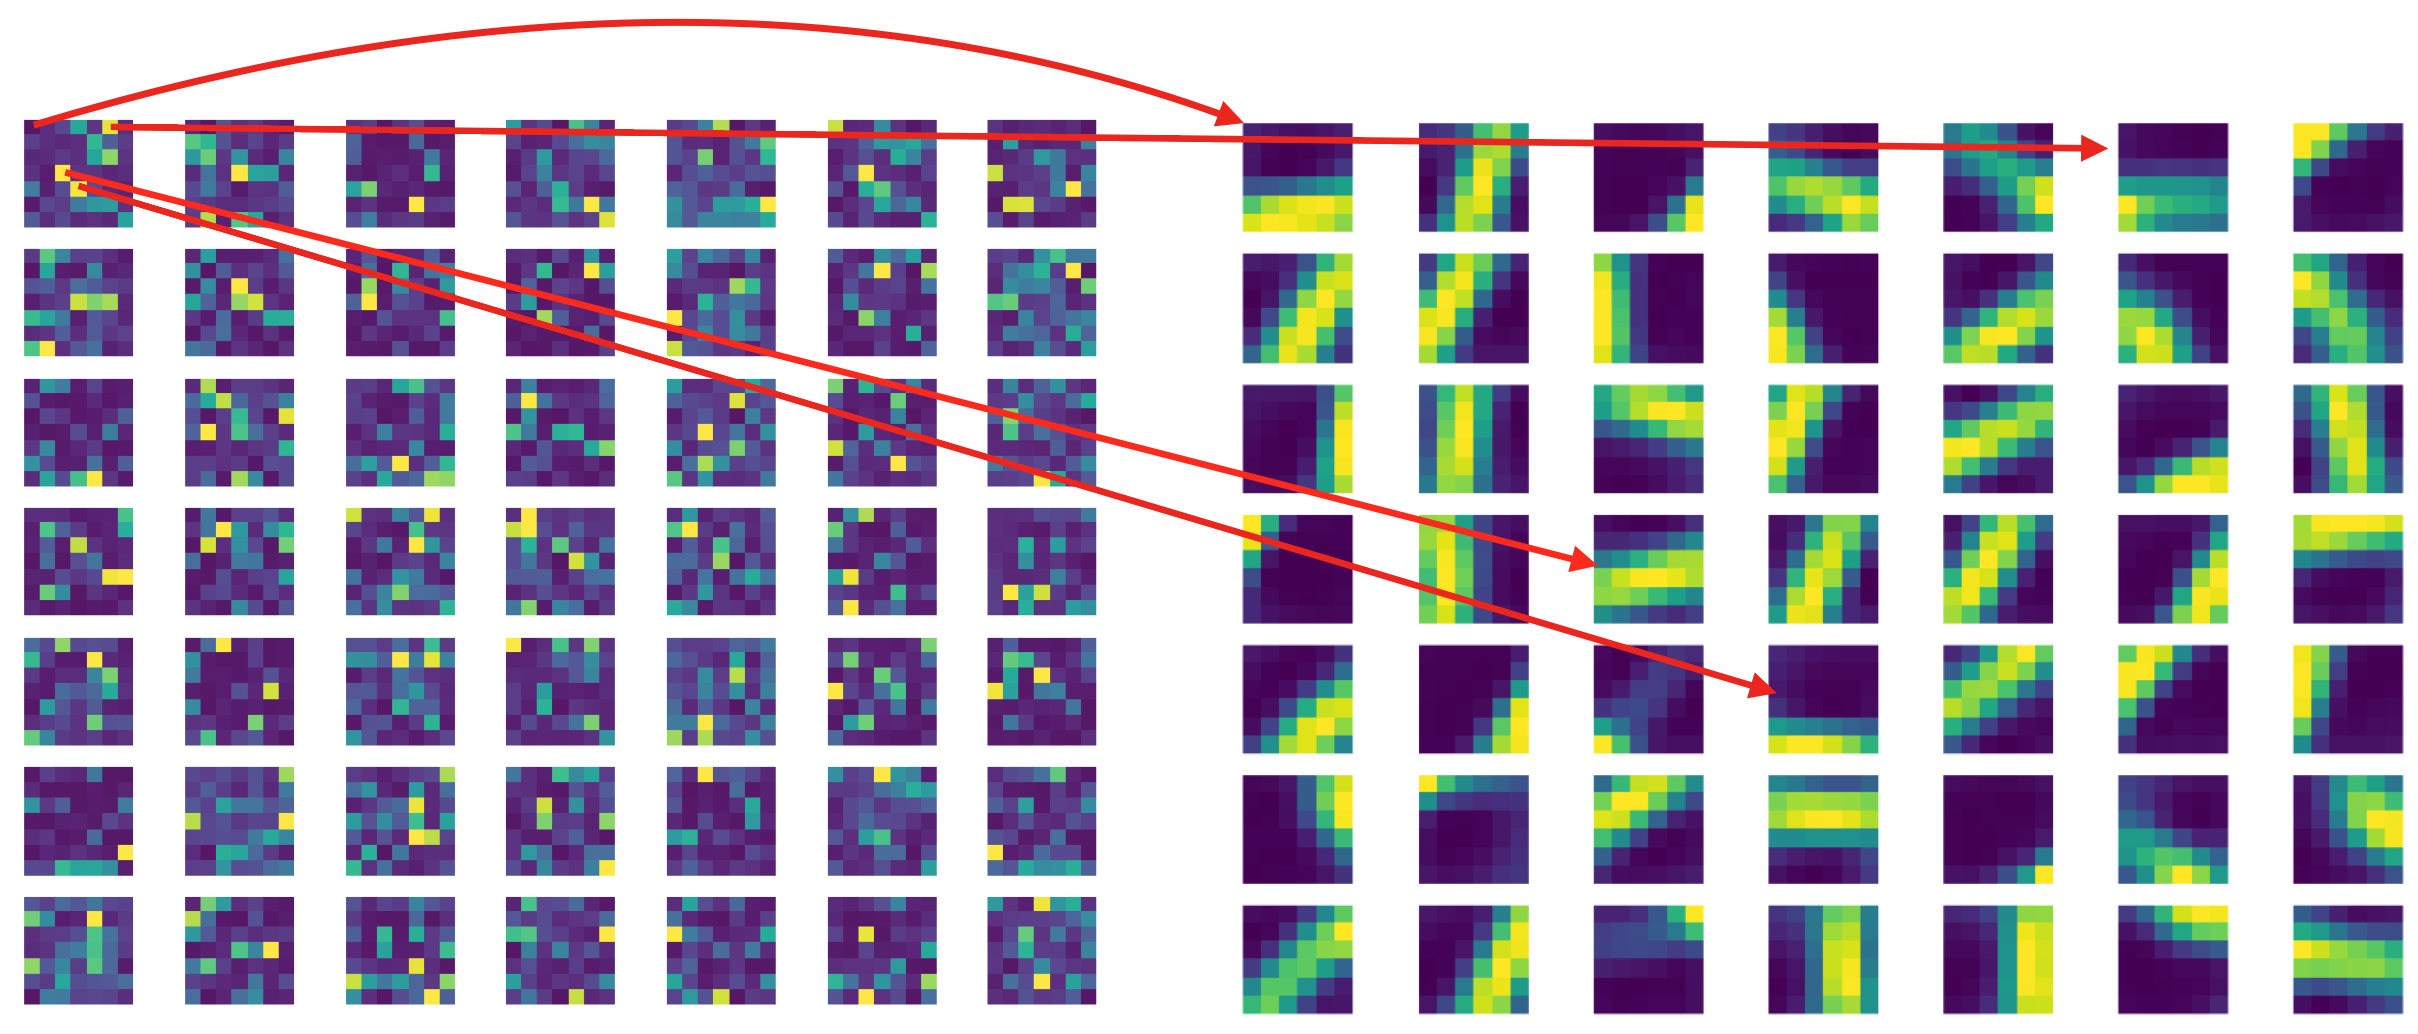
\includegraphics[width=13.8cm]{motor_drift}
	\caption{Receptive fields $p(\boldsymbol{x}|y_j)$ of 49 neurons (right) and correlation matrices (left) showing probability distribution $p(y_h^{(t+1)}|y_j^{(t)})$ over neighbouring cells. One pixel in correlation matrix corresponds to one neuron in the same column. One example has been marked with red arrows. All the bright pixels are connected by arrow to their corresponding field. All those fields happen to be vertical straight lines. It is possible to use such correlation matrices to find out which neurons are selective to the same feature but at different location. The loopback probability $p(y_j^{(t+1)}|y_j^{(t)})$ has been set to $0$ everywhere, because its not interesting to detect the same feature spiking in consecutive steps.}
	\label{fig:motor_drift}
\end{figure} 
It can be done by introducing layers with ``sticky'' activations. Those are neurons that remain active throughout all time steps, until enough motor feedback comes from outside and pushes the activations to change. The feed-forward input coming from lower layers is not ``strong'' enough to flip the activity pattern in the column.

In biological brains,  the ``sticky'' activations could be modelled using attractor states, strong cross inhibition or a mixture of both.
 

\paragraph{Benchmarks} In the figure \ref{fig:benchmarks} we present accuracy benchmarks on MNIST dataset. It compares the effects of using  motor feedback (viewport ``drift'') on different architectures. Two of them have been highlighted in green. Those are the exact same networks, except that one of them as additional layers with $d>1$. The $d$ variable in the stands ``drift'' and specifies how far away (in pixels) can the viewport be translated until the activation pattern in that layer changes. Until then, all the incoming input is associated with the current ``sticky'' winner neuron. 

The remarkable achievement is that the ``sticky'' layers with $d>1$ allow for significant reduction in number of channels. It forms a bottleneck, which forces the network to build translation-invariant abstractions of observed objects. If the motor feedback was even richer (allowing for head rotation, body movement, object manipulation etc.) then the networks would be able to learn about more complex semantic properties of the interactive environment.


\begin{figure}[!htbp]
	\centering
	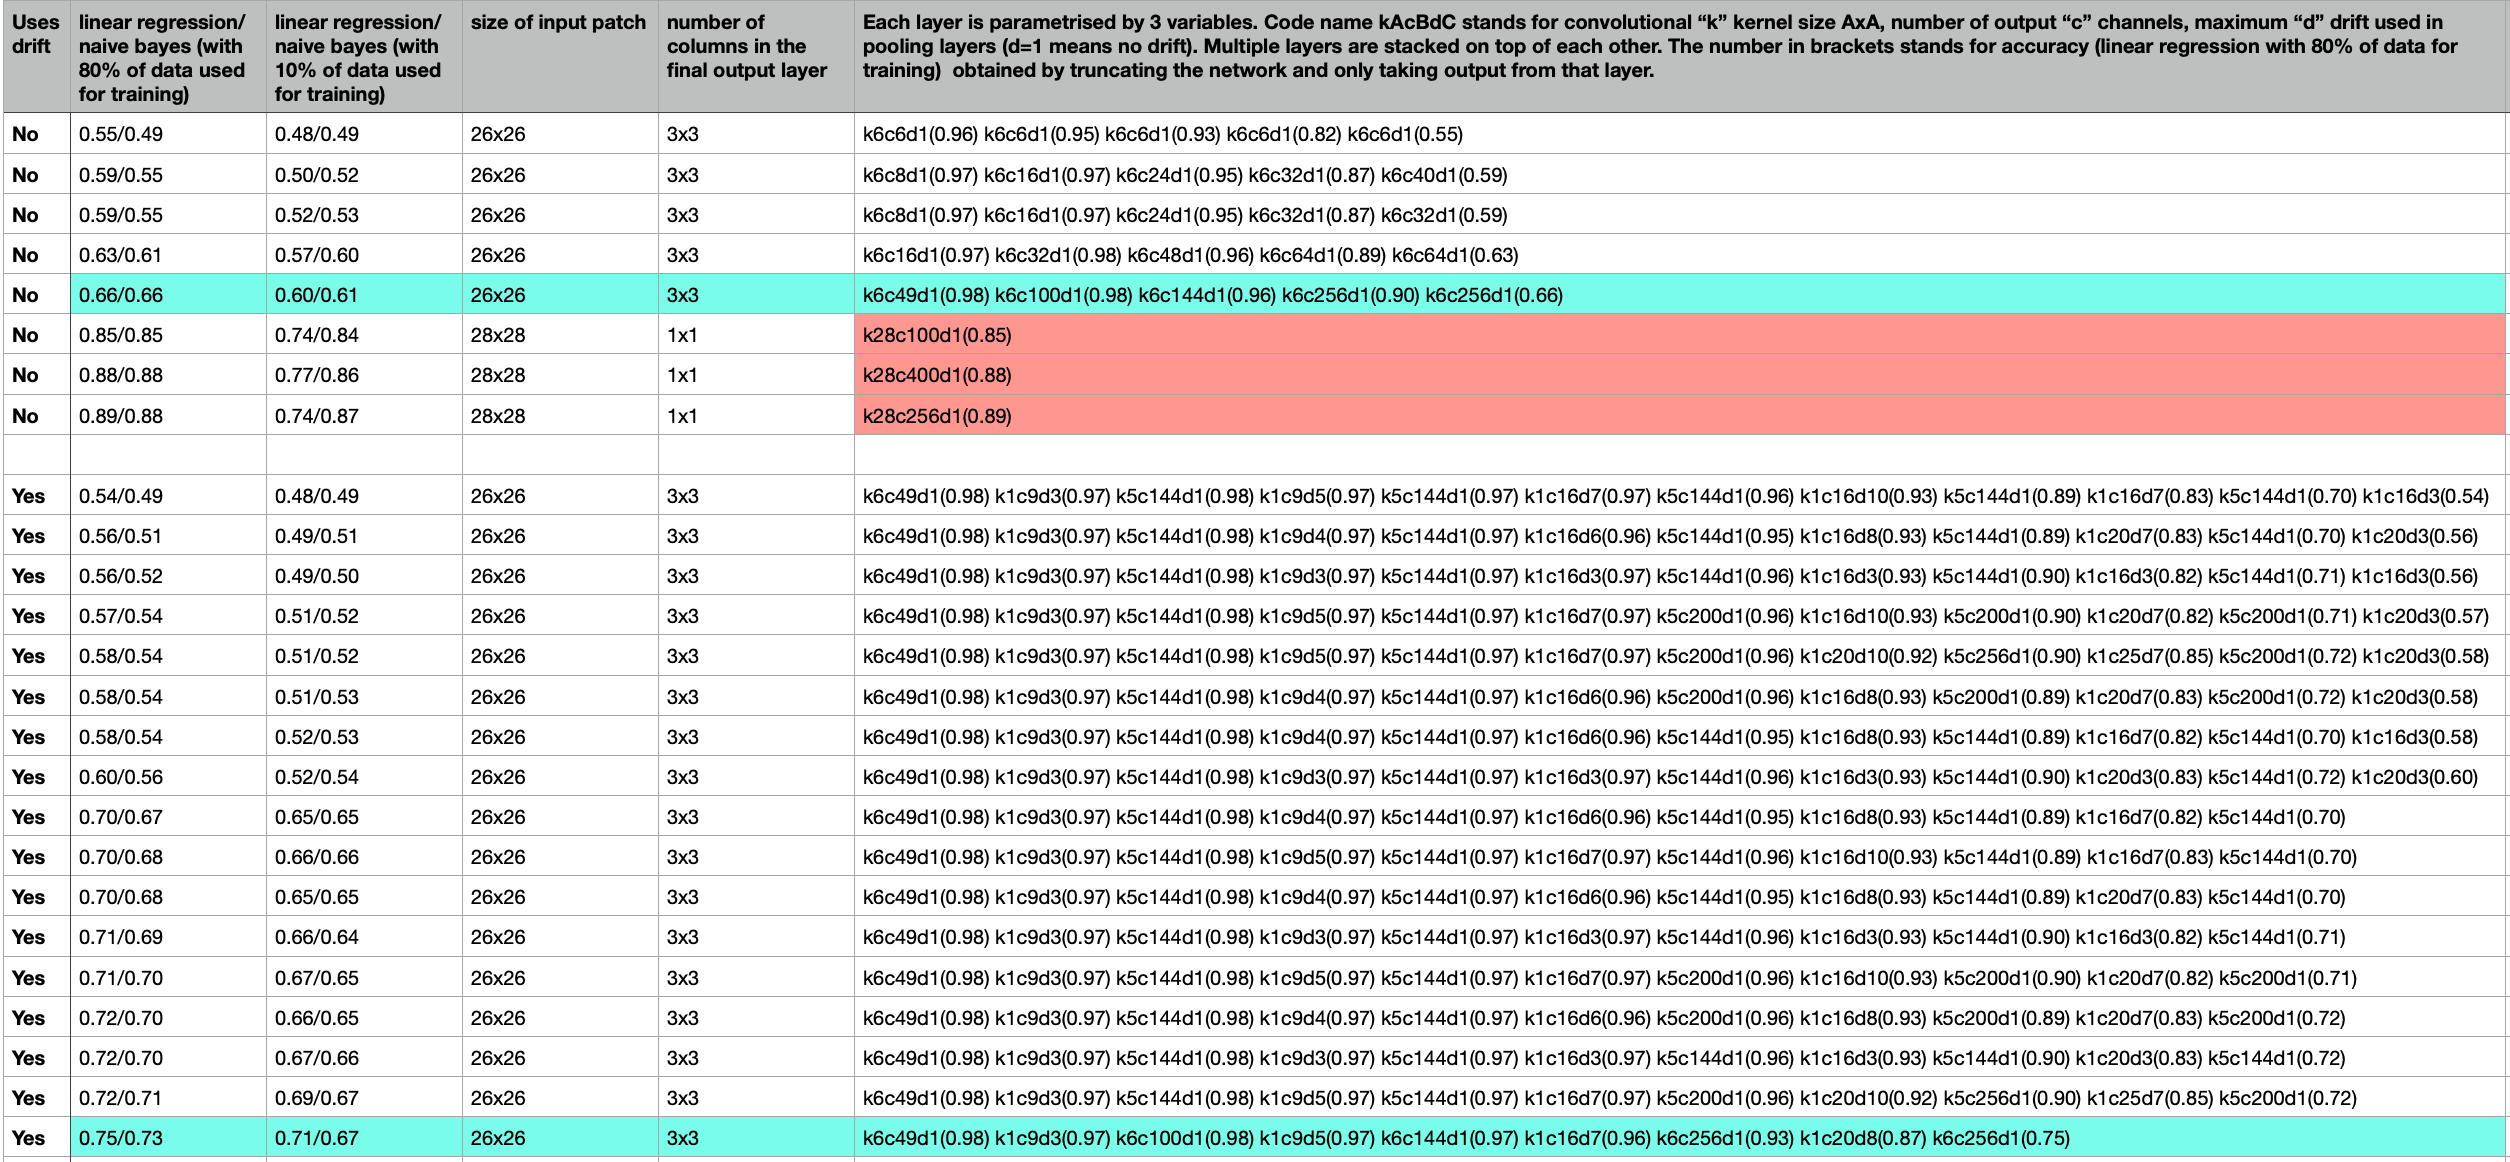
\includegraphics[width=13.8cm]{benchmarks}
	\caption{MNIST recognition accuracy benchmarks. The green rows mark two specific architectures that are nearly identical, except that one uses ``drift'' and has ``sticky'' layers with significant channel bottlenecks.  The red rows are shallow architectures without convolution (kernel $28\times28$ is equivalent to densely-connected layer), which show what happens when the number of channels grows}
	\label{fig:benchmarks}
\end{figure} 

Figure \ref{fig:benchmarks_votes} provides further details on the few architectures previously highlighted in colour. It shows accuracies of three classification strategies: linear regression, naive bayes and voting. While the first two have access to all bits from the final output layer, the last classification head is consists of many ``smaller heads'' - one for every column. Each one of them attempts to guess the label of MNIST digit based solely on activation pattern (one active bit) within a single column. At the end, whichever digit receives the most votes, wins. Such classifier is unable to take advantage of location information. 

\begin{figure}[!htbp]
	\centering
	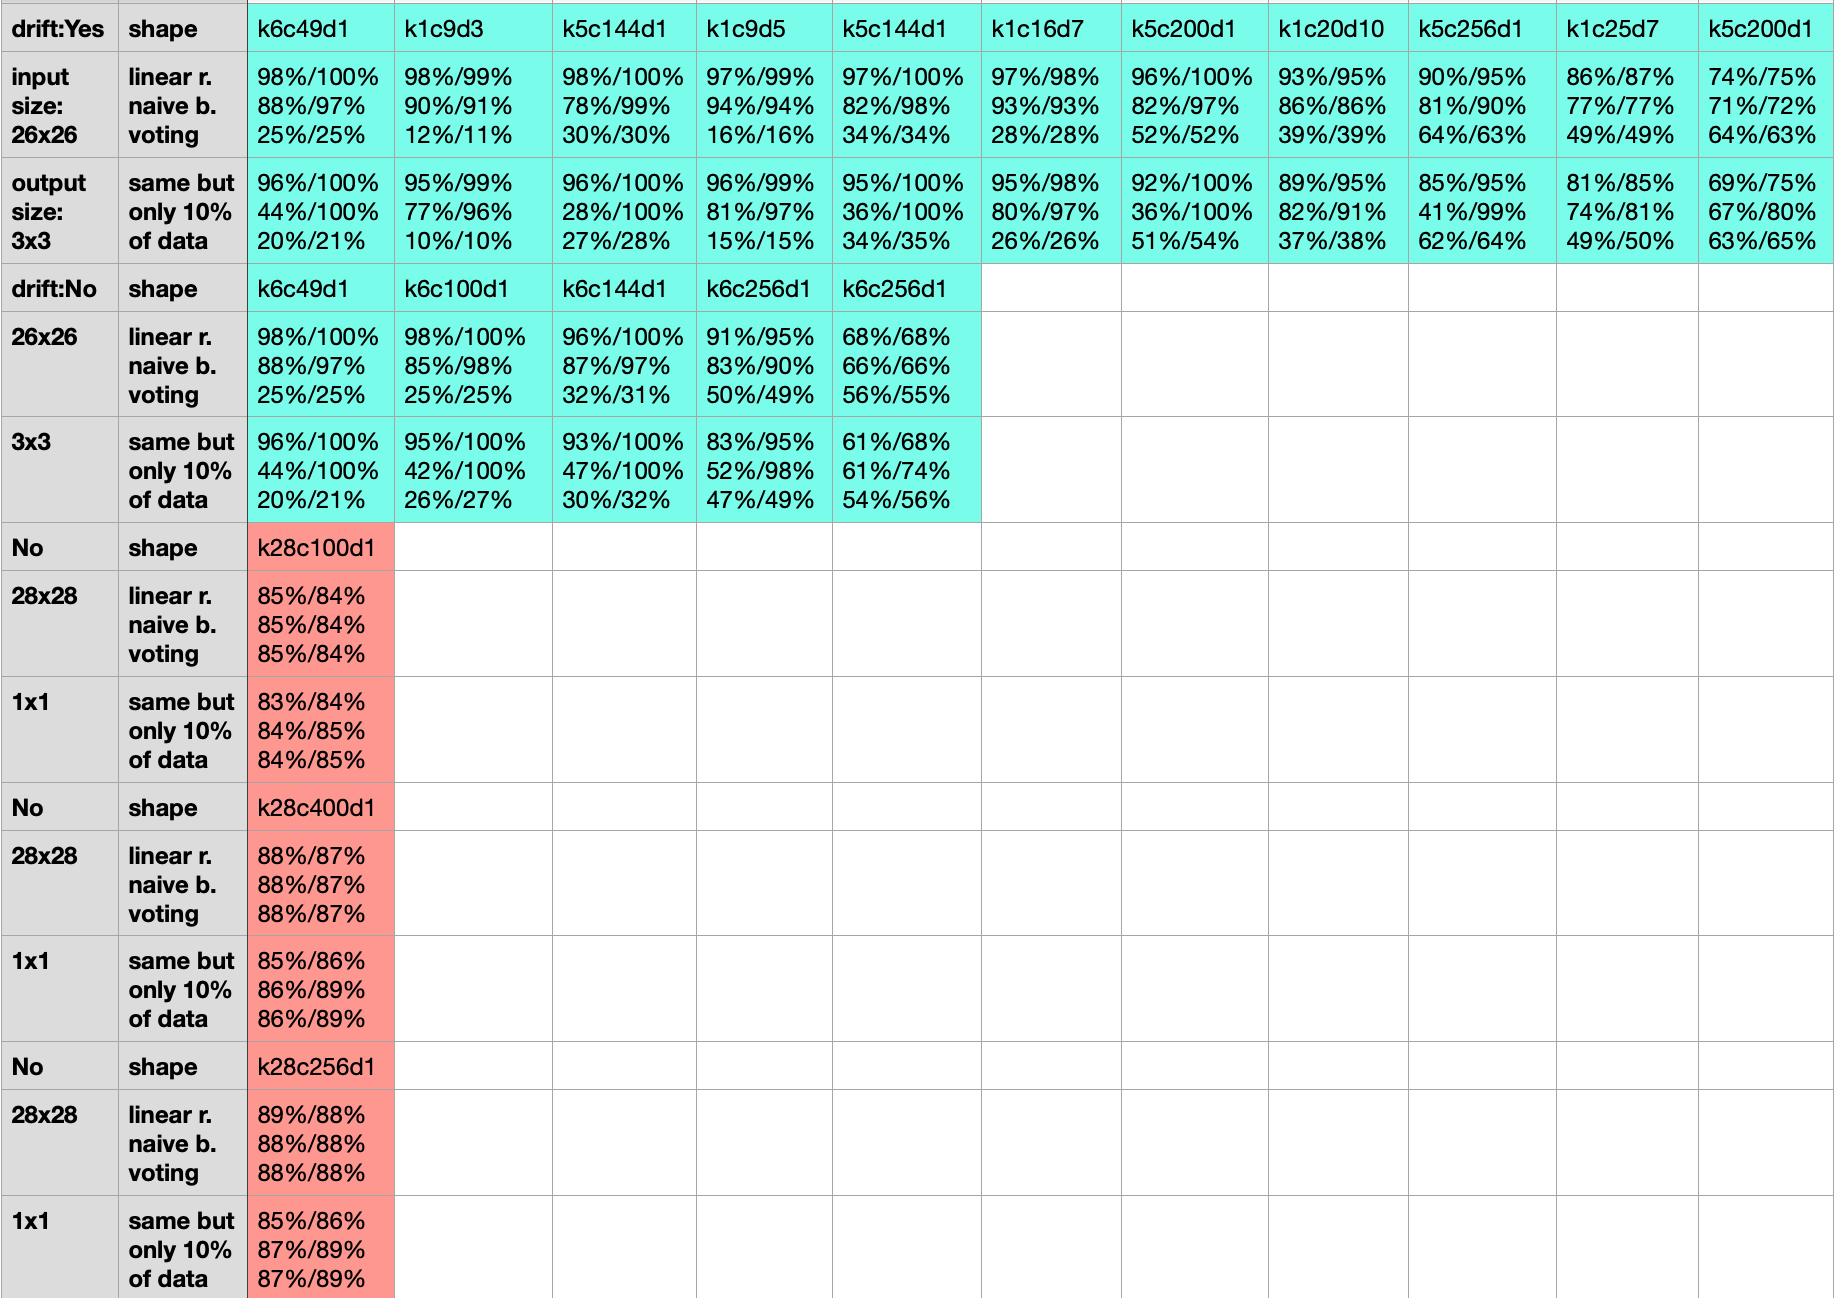
\includegraphics[width=13.8cm]{benchmarks_votes}
	\caption{The results are in the format of X\%/Y\%  where X stands for evaluation set and Y is for train set accuracy score.}
	\label{fig:benchmarks_votes}
\end{figure} 

\paragraph{Multiple bits per column} The topology of convolutional ECC networks can be extended to allow for more than 1 bit to appear in a single column. The only difference is that now there are several inhibitory neurons. The column is then divided into a few non-overlapping subpopulations such that all of the excitatory neurons within the same subpopulation are mutually exclusive (inhibited by the same neuron). The architecture marked previously in green, has layers with as many as 256 channels. This results in $0.03\%$ sparsity, which is much lower than the estimated $2\%-5\%$ in the real brain. By subdividing the columns the sparsity percentage can be raised. For example by subdividing a column with 100 channels into 4 subpopulations, the resulting sparsity is $\frac{1}{100/4}=\frac{1}{20}=5\%$. Figure \ref{fig:benchmarks_k} shows that the accuracy decreases. This is expected because now we are modelling $q(\boldsymbol{x}|y_j)$ with fewer coincidence classes $m$ allowing us for ``less resolution''. The surprising observations is that the decrease is very small and almost negligible (difference of around 1\%-2\%). That's because now  we are modelling $q(\boldsymbol{x}|y_{j_1},y_{j_2}...,y_{j_Y})$ using a product of  $q(\boldsymbol{x}|y_{j_1},y_{j_2}...,y_{j_Y})=q(\boldsymbol{x}|y_{j_1})q(\boldsymbol{x}|y_{j_2})...q(\boldsymbol{x}|y_{j_Y})$. 

\begin{figure}[!htbp]
	\centering
	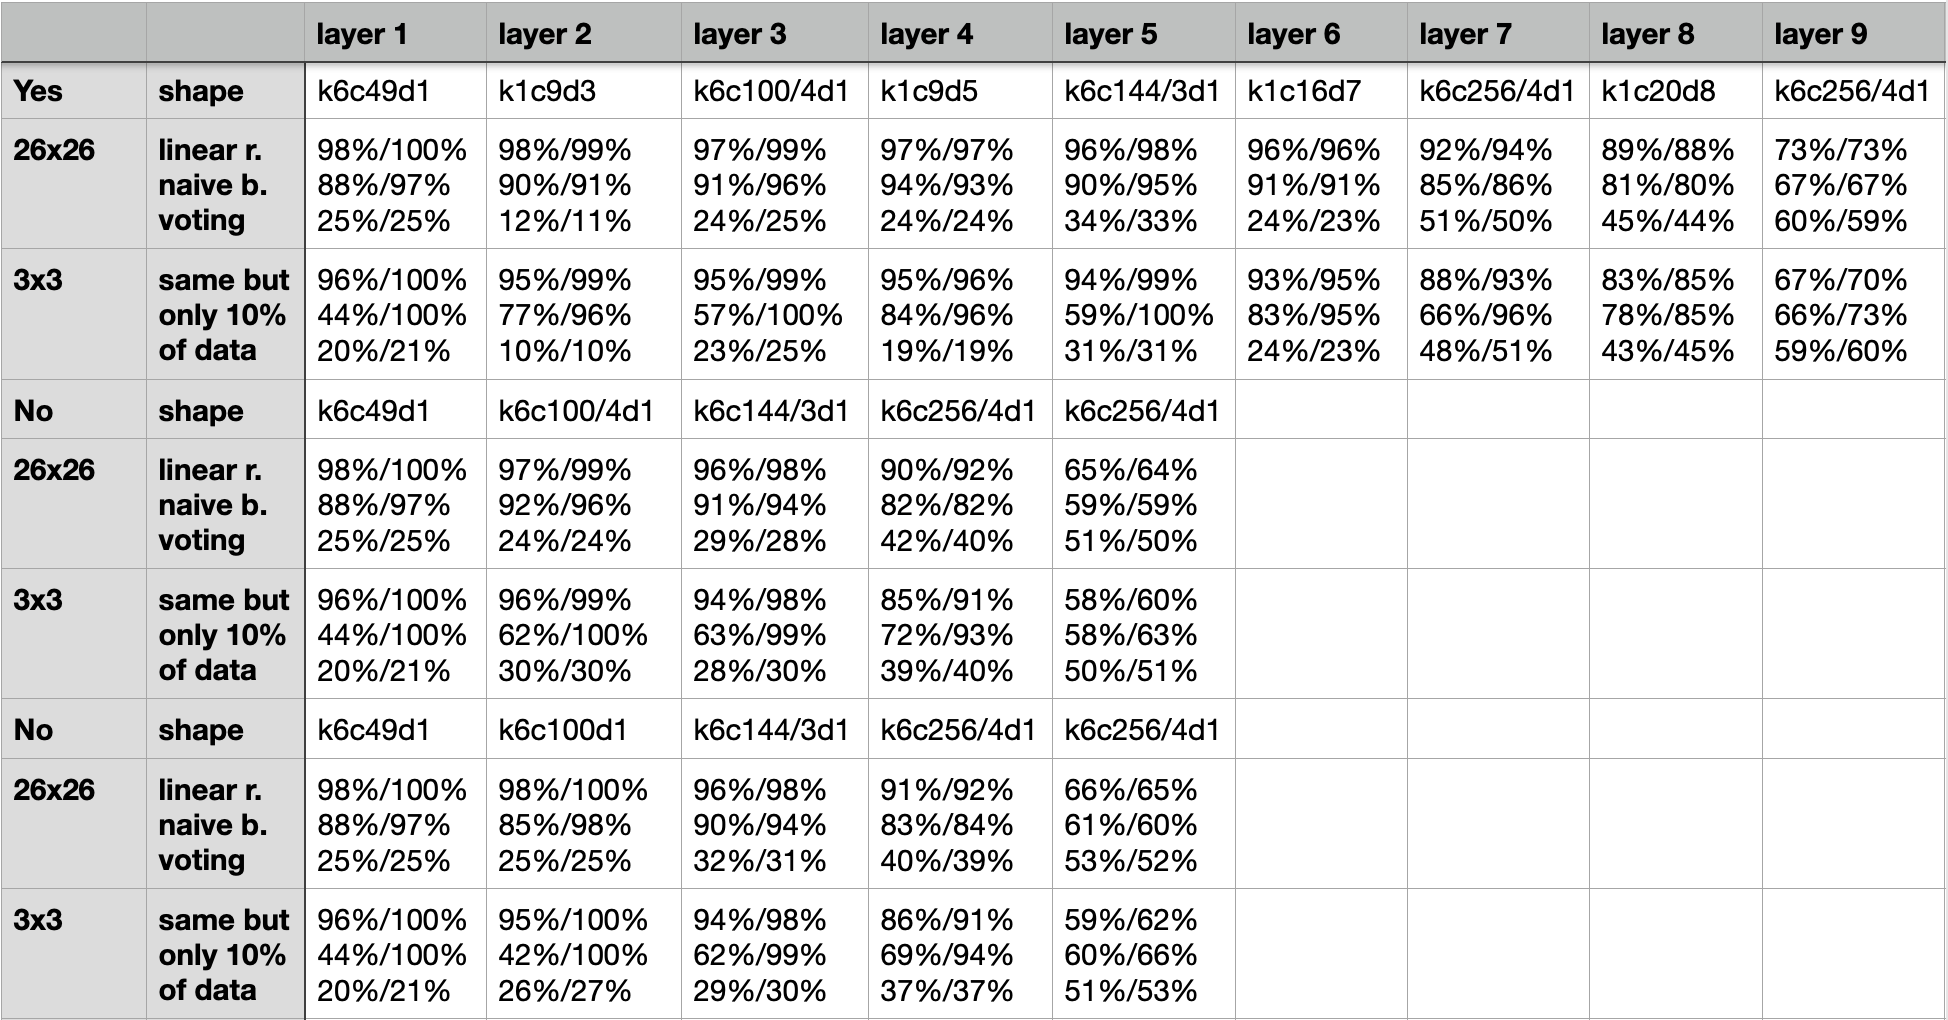
\includegraphics[width=13.8cm]{benchmarks_k}
	\caption{The layer topology is now marked with cX/Y which stands for X channels subdivided into Y populations. As a result there will be Y active bits per column. This table can be easily compared with figure \ref{fig:benchmarks_votes}.}
	\label{fig:benchmarks_k}
\end{figure} 

\paragraph{Sparse connections (dropout)} All of our ECC networks so far have used weight matrices $W$ representing dense connection. The real neurons are not so well organised. A far more biologically-plausible model can be achieved by randomly setting certain weights in $W$ to zero forever (hebbian learning is not allowed to modify them). 
Randomly dropping certain percentage of weights allows for building sparsely-connected networks where each neurons has access to only some fragment of the input. 

When we subdivide a column into several subpopulations, each one of them will have access to the same fragment of input. By adding dropout, we can introduce enough bias to prevent all of the subpopulations from becoming identical. This allows for additional regularisation.

Dropout combined with column subdivision is by far the most biologically accurate topology.

\paragraph{Deeper layers are less sensitive to small changes} 
Different layers have their own sensitivity to motor feedback. The lower ones are used to detect smaller features, like line patterns. Even small ``eve movement'' are enough to entirely change the detailed features, therefore the low layers should be more sensitive to small motor feedback. Deeper layers could be driven by motor-feedback neurons that activate in response to larger movements. For example, eve movement should not affect the more general landmarks in the surrounding environment, but head-direction could have a significant effect. As a result, the deeper  layers could learn to recognise increasingly more general concepts that change at broader scales of movement. 

\paragraph{Recurrent connections within columns}
The convolutional ECC networks are arranged in feed-forward layers and lack recurrent connections. Figure \ref{fig:recurrent_connections} shows what would happen if we added recurrent weights within each column. It becomes possible to model probability $p(y_h^{(t+1)}|y_j^{(t)})$. 

We empirically collected statistics of activation pairs $p(y_h^{(t+1)}|y_j^{(t)})$ in consecutive time-step and obtained a correlation matrix for every neuron in some column of a hidden layer. Throughout the experiment, no recurrent weights were present. Then we added recurrent connections within each column and trained them with hebbian learning. The weights have learned to model the exact same distribution, which can be seen on figure \ref{fig:recurrent_connections}.

\begin{figure}[!htbp]
	\centering
	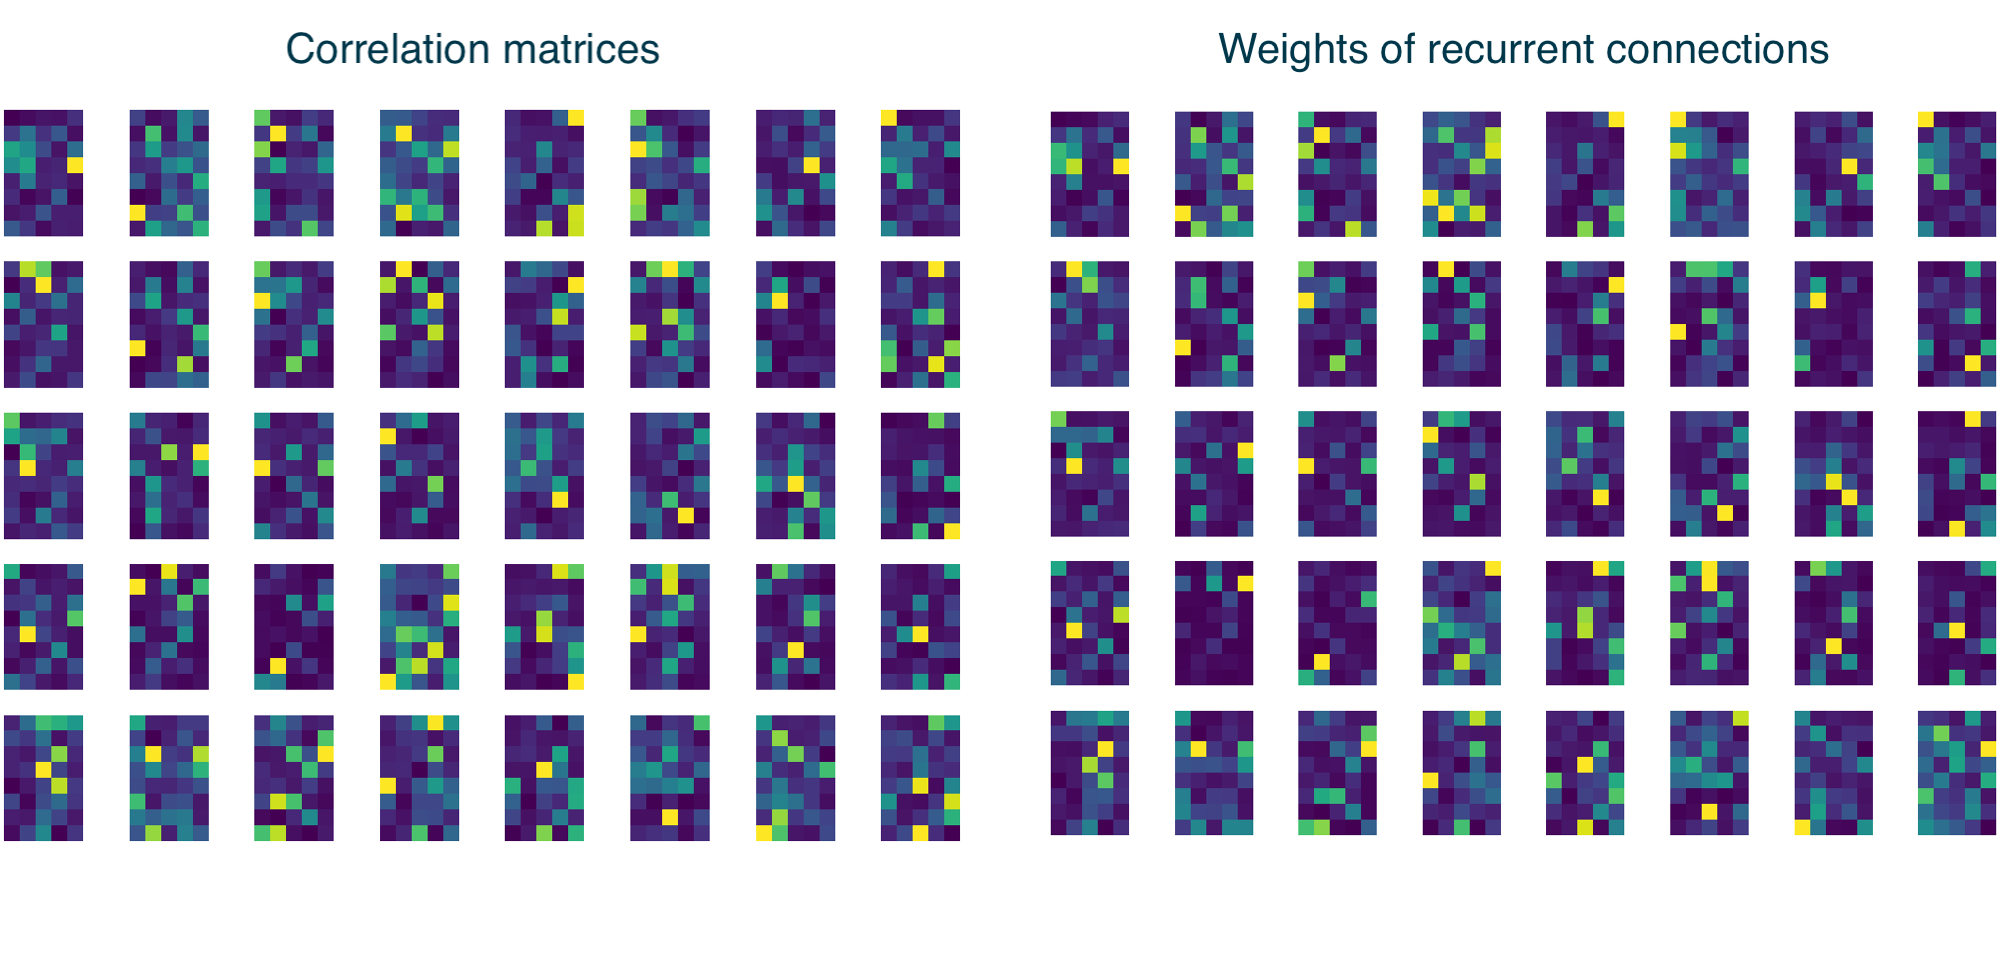
\includegraphics[width=13.8cm]{recurrent_connections}
	\caption{Recurrent receptive fields $p(\boldsymbol{y}^{(t)}|y_j^{(t+1)})$ of 40 neurons within the same column. Warmer colours mean higher values.}
	\label{fig:recurrent_connections}
\end{figure} 
 
 \paragraph{Voting and recurrent connections between layers}
 
 The mechanism of ``sticky'' activations can be elegantly combined with recurrent connections, the effects of which, resemble a ``voting'' mechanism, whose existence in the neocortex has been long speculated.
 
In the benchmarks from figure \ref{fig:benchmarks}, the layers with $d>1$ always used kernel size 1x1. This doesn't have to be the case. We could use larger kernel.  Then the sticky activation pattern in a column from higher layer will receive ``votes'' from nearby columns in lower layer. The sticky pattern will change only when the sum of input signal coming from lower layers is strong enough to override inhibition and force a different sticky activation to arise. The lower layers ``vote'' to change the higher ones. If the input activation is unexpected and each neuron predicts a different pattern, then the higher layer sticky activations won't change. 

If we also add recurrent connections going from higher layers back to lower, then such feedback signal could be used to train the lower layer activations. Such connectivity pattern will lead to self-organisation and reinforcement of predictable activations.

The motor feedback is no longer necessary but it could be possible to use it in combination with voting and recurrent feedback.

\section{Alternative models}

There exist several possible modifications. The columns $W_j$ of weight matrix must sum up to $1$. In other words the $\ell_1$ norm is $\lVert W_j \rVert_1=1$.
What would happen if we used $\ell_2$ norm instead?

Then all columns of $W$ matrix are unit vectors. The inner product $\boldsymbol{x}W_j$ measures cosine similarity 
\[
\boldsymbol{x}W_j = \lVert \boldsymbol{x} \rVert_2 \lVert W_j \rVert_2 \cos \theta = \lVert \boldsymbol{x} \rVert_2 \cos \theta 
\]
The inequality $\boldsymbol{x}W_h \ge \boldsymbol{x}W_j$ implies that angle between $\boldsymbol{x}$ and $W_h$ is smaller than that between $\boldsymbol{x}$ and $W_j$. 
\begin{gather*}
	d(\boldsymbol{x},W_j )= \arccos(\frac{\boldsymbol{x}}{\lVert \boldsymbol{x} \rVert_2}W_j)\\
\boldsymbol{x}W_h \ge \boldsymbol{x}W_j \implies d(\boldsymbol{x},W_h) \le d(\boldsymbol{x},W_j)
\end{gather*}
If we imagine $W_j$ to be a point on n-dimensional sphere $S^n$, then $\frac{\boldsymbol{x}W_j}{\lVert \boldsymbol{x} \rVert_2}$ can be used to measure geodesic distance between $\boldsymbol{x}$ and $W_j$. Such ECC networks could be reformulated as a k-means algorithm that operates on topology of a sphere, rather than Cartesian coordinates. By taking $\argmax(\boldsymbol{x}W)$ we select the point $W_j$ that lies closest to  $\frac{\boldsymbol{x}}{\lVert \boldsymbol{x} \rVert_2}$.
Each neuron $y_j$ represents a cluster $C(y_j)$ of all the points $\boldsymbol{x}$ whose geodesic distance is closest to $W_j$. The centroid $\mu(y_j)$ of cluster $C(y_j)$ is defined as Karcher mean
\begin{gather*}
C(y_j) = \{\boldsymbol{x}:\argmax(\boldsymbol{x}W)=j\} \\
\mu(y_j) = \argmin_{W\in S^n} \sum_{\boldsymbol{x}\in C(y_j) } d(\boldsymbol{x},W)^2 \bar{p}(\boldsymbol{x}|y_j) = \argmin_{W\in S^n} \mathbb{E}_{\bar{p}}\big(d(\boldsymbol{x},W)^2\big|y_j\big)
\end{gather*}
In the general case the centroid $\mu(y_j)$ may not be unique. For example the Karcher mean of two antipodal points $\boldsymbol{x}=-\boldsymbol{x}'$, could be any point on the equator. In the specific case of ECC networks, all of the inputs $\boldsymbol{x}$ are binary vectors $\{0,1\}^n$, hence we only operate on the positive fragment of a sphere. Here the mean $\mu(y_j)$ is always unique and it coincides with the normalized arithmetic mean (one that uses euclidean distance instead of geodesic).
\[
\mu(y_j) = \frac{}
\]



Figure \ref{fig:benchmarks_l2} presents benchmarks that compares MNIST accuracy of networks trained with $\ell_1$ and $\ell_2$ norms.


\begin{figure}[!htbp]
	\centering
	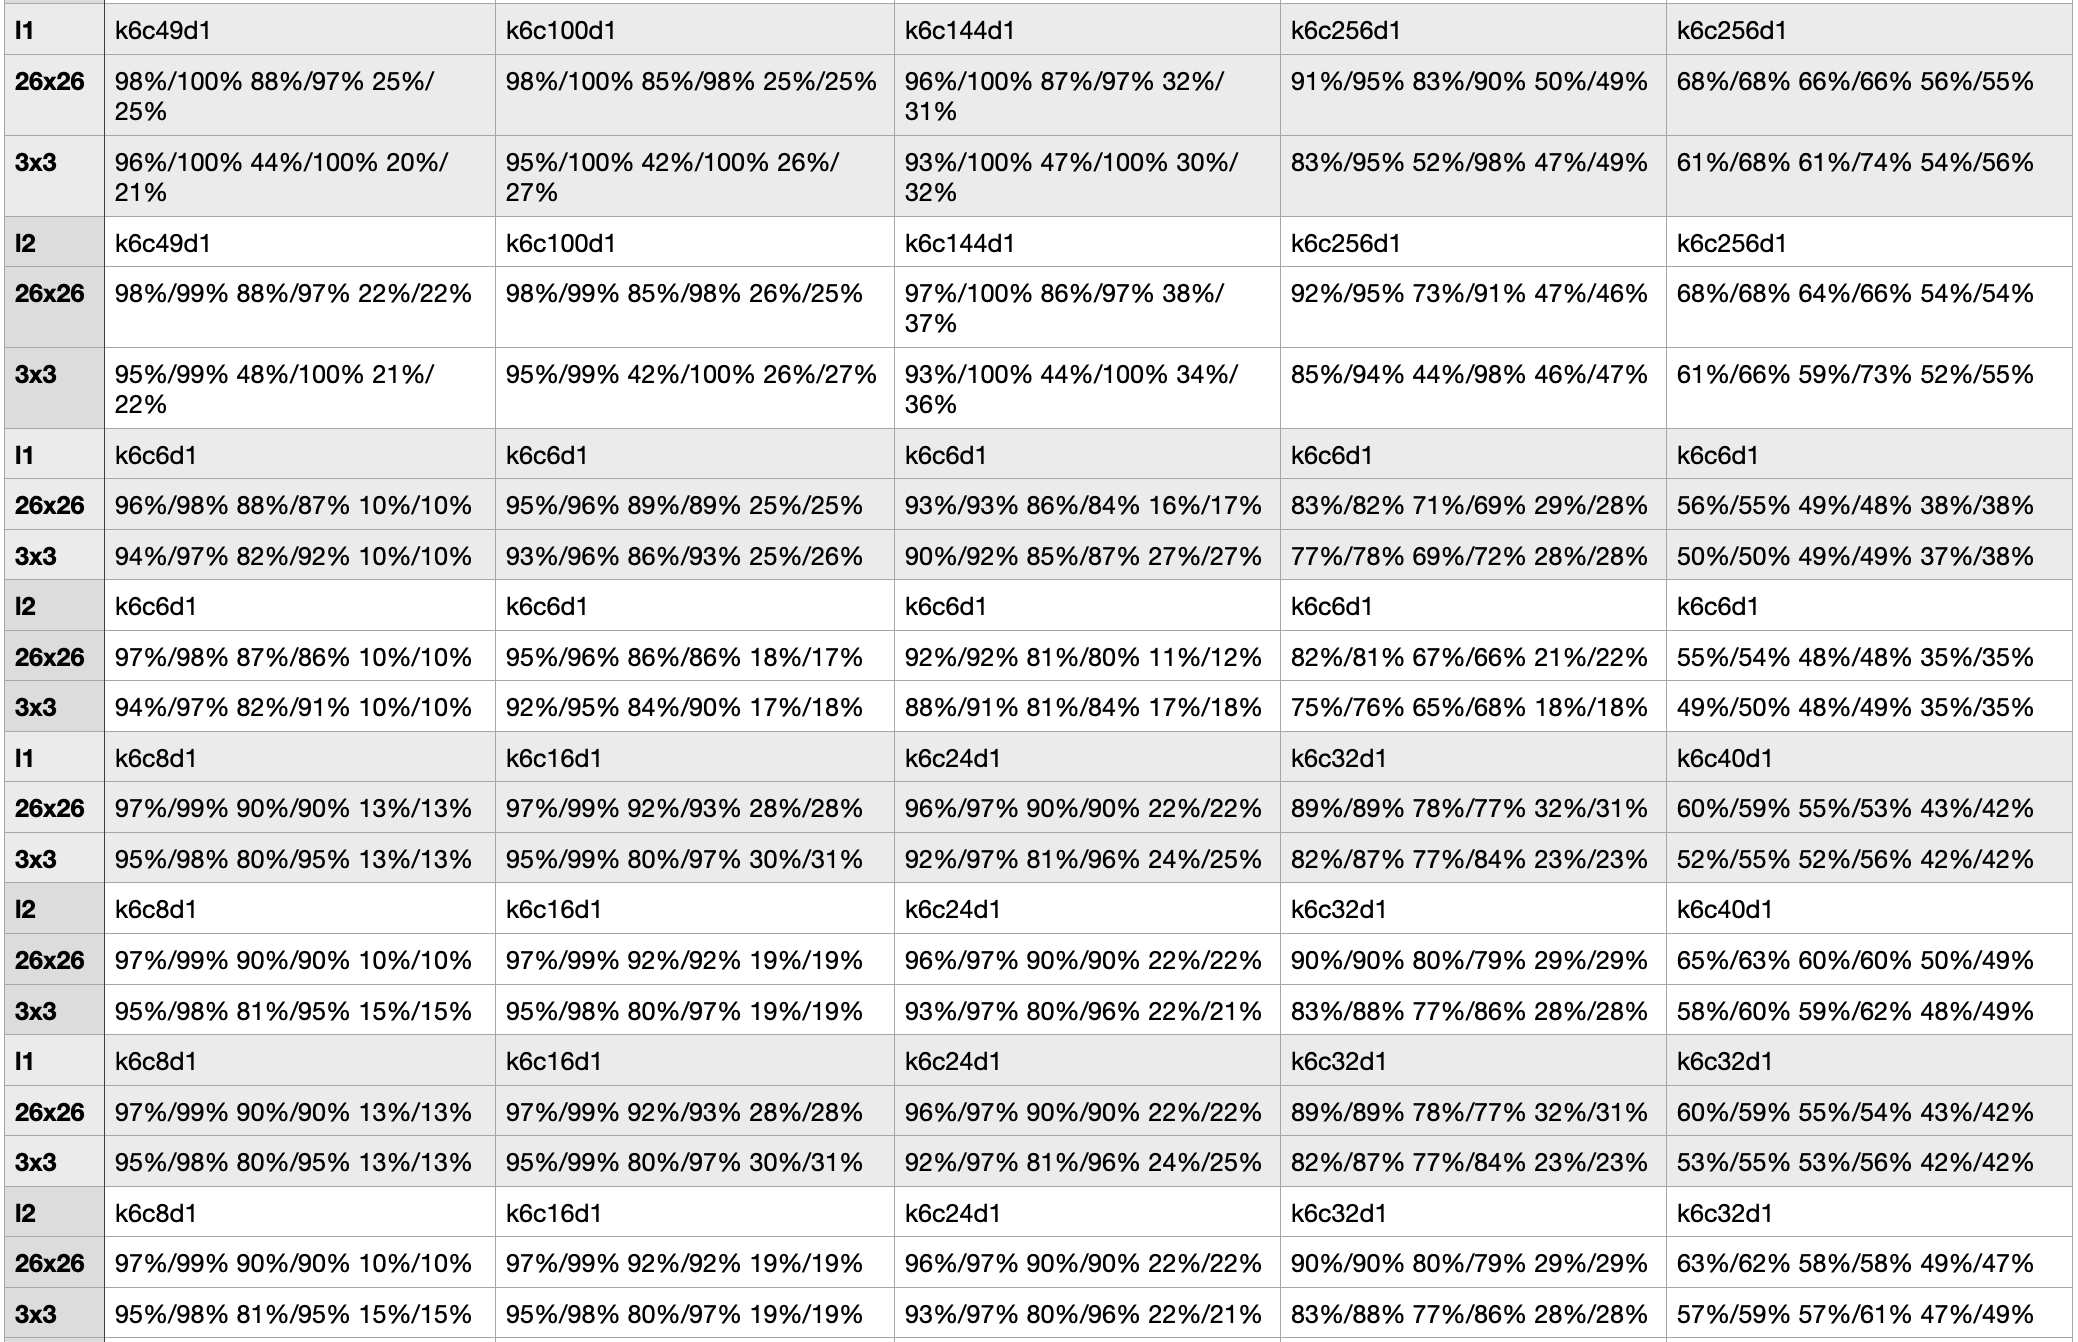
\includegraphics[width=13.8cm]{benchmarks_l2}
	\caption{Comparison of benchmarks using $\ell_1$ (grey) and $\ell_2$ (white) metrics.}
	\label{fig:benchmarks_l2}
\end{figure}

 
\section{Reinforcement learning and control}

\paragraph{ECC can't learn value functions}

The deep neural networks learn using backpropagation. They are inherently a supervised method of building intelligence. Even when the labels and error comes from the data itself, like in the self-supervised approach, the learning algorithm itself still relies on the same supervised mechanisms. Deep nets can be applied to reinforcement learning problems by modelling the reward function. ECC networks on the other hand are purely unsupervised and they do not approximate functions. They can't represent policy or reward function in the same way as deep nets. However, the biological brains are capable of performing control tasks very well. How could we achieve the same using ECC networks?

\paragraph{Geometric deep learning theory}

In order to see how ECC networks can solve control tasks, we need to first understand why deep learning works so well and why deep reinforcement learning is different from all other modalities. 

Geometric deep learning provides a mathematical framework and theory for understanding deep nets. The task is to find a function $f:\mathcal{X}\rightarrow\mathcal{Y}$ that belongs to some parameterised function class $\mathcal{F}=\{f_{\theta \in \Theta}\}$, where $\theta$ are typically the weights of a neural network. The set $\mathcal{X}$ is some high-dimensional input space $\mathcal{X}=\mathbb{R}^n$. The learning process attempts to find some $f_\theta$ that fits well into an observed set of samples $\mathcal{D}=\{(x_i,y_i)\}_{i=1}^N$. Identifying such a function is difficult due to curse of dimensionality. The number $N$ of necessary samples grows exponentially with the dimensionality $n$. In order to overcome this obstacle, deep nets use geometric priors. They assume existence of symmetries in the signal space. Each signal $x$ is a function $x:\Omega \rightarrow \mathcal{C}$ where $\Omega$ is called the domain and $\mathcal{C}$ is the value.
For example a neural network that operates on 28x28 images with RGB pixels will receive signals $x:\mathbb{Z}_{28}\times \mathbb{Z}_{28} \rightarrow \mathbb{R}^{3}$. The signals form a Hilbert space and a linear space. Symmetries in $\Omega$ are defined by some group $\mathcal{G}$, whole elements $g\in \mathcal{G}$ act on domain $\Omega$. Group actions on signals are defined as $(g.x)(\omega)=x(g^{-1}\omega)$. For example computer images can be translated under the group of 2D translations acting on pixel coordinates $\mathbb{Z}_{28}\times \mathbb{Z}_{28}$. Deep network architectures allow constraining the search space $\mathcal{F}$ to include only functions that are invariant ($f(g.x)=f(x)$) or equivariant ($f(g.x)=g.f(x)$) under transformations of a specific group. This counters the curse of dimensionality and allows for identifying functions with less than exponential number of samples.

\paragraph{Reinforcement learning sample inefficiency}
While most modalities, such as computer vision, natural language, audio/speech recognition are largely considered to be ``solved'', reinforcement learning is the last frontier where deep networks still struggle. We have seen impressive results such as AlphaGo beating the world's champion in Go, but at the same time, those achievements were only possible by using immense amounts of training time and computing power. It appears as though reinforcement learning is in some sense ``different''. Could it be that control tasks have some unexplored hidden symmetries? What kind of deep network architecture could solve the curse of dimensionality and allow for efficient reinforcement learning?

We propose that the missing symmetries are not in the inputs signal $x$, but in the actions that the agent can take. An agent moving 2 steps forward and 2 steps backward will end up in the same place. An agent rotating $360\deg$ around itself, will end up facing the same direction. Moving your hand 15cm up and 15cm down will not result in any change. 

\underline{Neuroscientific hypothesis}: The biological brains are capable of learning action symmetries and the results can be observed in form of head-direction cells and grid cells. We predict existence of cells coding many other group symmetries. For a long time it has been suspected that the hippocampus learns graphs. We propose that those are not just any graphs. They should be Cayley graphs generated by agent's actions. If our hypothesis is true, then it would be rather likely that the human language has evolved as a result of building higher and more sophisticated group abstractions of the real world. 
\iffalse Every word of human language might be bound to some element of that group. 
Many of those elements might commute. For example all of the following sentences, even though not grammatically correct, are understandable and their ``common sense'' meaning is the same: ``I ate duck'', ``ate I  duck'', ``ate duck I'', ``duck I ate''. This would agree with the fact that transformer architectures (deep nets modelling class of permutation-equivariant functions) are so good at processing natural language. 
\fi

\paragraph{Inference of groups from actions and observations}

Geometric deep learning theory can be modified to learn groups $\mathcal{G}$ instead of functions $\mathcal{F}$. Let $\mathcal{A}$ be a generator set of $\mathcal{G}$. The network is presented with a trajectory 
\[x_1,g_1,x_2,g_2,x_3,g_3... \text{ such that } \forall_{t>0} g_t \in \mathcal{A}\] 
of alternating actions and signals. The structure of $\mathcal{G}$ is not known to us. We only see the generating set $\mathcal{A}$, which is known in advance, but we can never observe any other group element. We attempt to infer  $\mathcal{G}_\theta$ under the assumption that  it belongs to some parametric family $G=\{\mathcal{G}_{\theta\in\Theta}\}$. The goal is to find some $\mathcal{G}_\theta$ such that the following holds 
\[
\exists_{ g_0\in\mathcal{G}_\theta} \forall_{t>0} g_t...g_2g_1g.x_0 = x_{t+1}
\] The observation $x_0$ is considered to be the initial state of the agent, before it has observed any signal. The initial $g_0$ is called the ``anchoring point'' and it determines how $x_1$ relates to the initial $x_0$. As a result, the learned group $\mathcal{G}_\theta$ must be able to explain how the agent got to the staring $x_1$. 

\underline{Neuroscientific motivation}: The grid/hd/place cell patterns are stable. There must exist some mechanism for anchoring them to the observed cues. If we did not use $g_0$ and $x_0$, then there might exist multiple possible $\mathcal{G}_\theta$ fitting the trajectory and any one of them could be chosen randomly. The pattern stability is ensured, because agent can use the first observation $x_1$ (cues) to infer $g_0$.
There is also one additional benefit. The learning algorithm should be capable of imagining the first $x_1$ based only on ``made up'' scenario $g_0$. It should also be able to recall past experiences by replaying them from a specific starting $g_0$.

\paragraph{Parametric groups}

There might exist many possible ways to parameterise structure of a group. Any finitely generated group can be defined using a set of word equivalences and then new equalities can be found using Knuth-Benedix procedure. Differentiable encoding can be achieved with real vectors $\mathbb{R}^n$ and then deep network could be trained by modelling the differentiable (Lie) group operations. Such encodings can be observed to emerge in Tolman-Eichenbaum machine. 

ECC networks allow for yet another group representation using sparse binary vectors. 
Every group element $g_{\boldsymbol{x}}$ is represented as a set of neurons (bits in binary vector) $g_{\boldsymbol{x}}=\{i:x_i\in\boldsymbol{x}\}$. Network connections  $W$ represent edges in Cayley graph. Such encoding allows for certain degree of imprecision and fuzziness. We can measure similarity of nodes by the overlap in their binary vectors. This allows for robustness when observations $\boldsymbol{x}$ are noisy.


Learning parametric groups has many analogies to inductive grammatical inference (learning finite state automata). We could represent any group using its Cayley graph and then try to minimise it by merging certain group elements with equivalence relations. The goal would be to find the minimal quotient group such that its actions on signals $\boldsymbol{x}$ are preserved (consistent with the observed trajectory). 

Consider a graph with $\omega$ vertices and an agent walking on it. Knowing the exact vertex where the agent is currently located, is equivalent to $\log_2 \omega$ bits of information. Anybody who ever attempted to model complex real-world systems using state graphs, would promptly notice that the number of required vertices $\omega$ is very large. The states representing real world may depend on many different latent variables $\boldsymbol{z}$ that by themselves carry $\lVert \boldsymbol{z} \rVert_1$ bits of information. Representing all possible configurations of those latent variables would exponentially require $\omega=2^{\lVert \boldsymbol{z} \rVert_1}$ states in the graph. Information carried by each state would be $\log_2 \omega=\lVert \boldsymbol{z} \rVert_1$ bits.


In classical reinforcement learning, the agent occupies a specific state in a Markov decision process (MDP). It is assumed that the agent knows exactly where it is at any point in time. Deep reinforcement learning generalises MDP by working with partially observable states. Such agents do not know the state and can only see certain representations $\boldsymbol{x}$ of it instead (like images).

Here we assume that the environment is a (very large or infinite) group $\mathcal{G}_*$ whose elements $g_{\boldsymbol{z}}$ are the states. Every state carries $\boldsymbol{z}$ bits of information. There exists a projection  $\mathcal{X}(g_{\boldsymbol{z}})=\boldsymbol{x}$ that produces observations of any given state. The information carried by $\boldsymbol{x}$ may be less than that of $\boldsymbol{z}$ (agent will have to infer missing bits from the trajectory). Agent acts on signal $\boldsymbol{x}$ with group-generating element $g_a\in \mathcal{A}$. The result of action is $g_a.\mathcal{X}(g_{\boldsymbol{z}})=\mathcal{X}(g_ag_{\boldsymbol{z}})$. 

The input to first layer in ECC network is the signal $\boldsymbol{x}$, while its output $g_{\boldsymbol{y}}\in\mathcal{G}_{\theta}$ is an approximation of $g_{\boldsymbol{z}}\in\mathcal{G}_{*}$. 

\paragraph{Inductive inference of groups}

It is possible for two different group elements $g_{\boldsymbol{z}}\ne g_{\boldsymbol{z}'}$ to produce the same observation $\mathcal{X}(g_{\boldsymbol{z}})=\mathcal{X}(g_{\boldsymbol{z}'})$, but assume that the probability of it is low. We first make certain simplification and assume that $\mathcal{X}$ function is deterministic. In the latter paragraphs we will generalise our conclusions to probabilistic and noisy observations.

Having sampled a trajectory
\[\boldsymbol{x}_1,g_1,\boldsymbol{x}_2,g_2,\boldsymbol{x}_3,g_3...\boldsymbol{x}_T\] 
we may attempt to infer the group's Cayley graph by greedily merging those observations $\boldsymbol{x}$ that are equal. This approach is similar to the RPNI (regular positive negative inference) algorithm used for inference of finite state automata (FSA). Any Cayley graph could be interpreted as FSA, while the generator $\mathcal{A}$ is analogous to the alphabet of a formal language. In our case, we assume that every state produces observations, which could be interpreted as finite state Moore machine. 

The inference algorithm is as follows. For every observation $\boldsymbol{x}$ in trajectory, let us create a corresponding vertex $g_{\boldsymbol{x}}$. Initialise the Cayley graph $\mathcal{G}_{\theta}$ so that every $g_{\boldsymbol{x}_t}$ and $g_{\boldsymbol{x}_{t+1}}$ is connected with an edge. Label the edges accordingly with their respective actions $g_{t}\in\mathcal{A}$. As a result, the initial  $\mathcal{G}_{\theta}$ graph will be a path. Then execute the following procedure
\begin{lstlisting}
for $t$ from 1 to $T$:
    for $t'$ from 1 to $t$:
       if $\boldsymbol{x}_t=\boldsymbol{x}_{t'}$:
           $\mathcal{G}_{\theta}'$  = copy of $\mathcal{G}_{\theta}$ 
           merge $g_{\boldsymbol{x}_t}$ with $g_{\boldsymbol{x}_{t'}}$ in $\mathcal{G}_{\theta}'$
           if cascade($\mathcal{G}_{\theta}'$):
                $\mathcal{G}_{\theta}$  = $\mathcal{G}_{\theta}'$   // update Caley graph  
\end{lstlisting}
The cascade procedure will attempt to iteratively merge all of the edges that have the same source vertex and are both labelled with the same action $g_{t}\in\mathcal{A}$. Before merging any two edges, their destination vertices are checked for ``compatibility''. They must produce equal observations $\boldsymbol{x}$. Such equality needs to be ensured because we assumed $\mathcal{X}$ to be deterministic. If the cascade attempt to merge two incompatible edges, then the procedure terminates with output $0$. If the iteration ends (there are no more candidate edges to merge), then the output is $1$. All merging operations are performed ``in-place'' and the graph  $\mathcal{G}_{\theta}'$ is mutated.

It can be shown that such procedure will always identify the correct Cayley graph in the limit as trajectory length $T$ approaches infinity (proof is the same as for Moore-RPNI algorithm).





\paragraph{Group manifolds}


Define a distance metric $d_L(g_1,g_2)$ on $\mathcal{G}$ generated by $\mathcal{A}$ as the minimum length of word $g_3$ such that $g_3g_1=g_2$. The $L$ in $d_L(g_1,g_2)$ stands for multiplying $g_3$ on the left side of $g_1$ (group elements  need not commute). 
We can use such metric to induce topology of open balls on $\mathcal{G}$.
%(If $\mathcal{G}$ is also differentiable then it's a Lie group, but we're not concerned with this here).

Within the open ball, a group might look different than elsewhere. For example movement of an ant inside a box might look like a group of two-dimensional translations, until it hits a wall. 



The latent group $\mathcal{G}_{*}$ might be large and complex. Learning can be made more efficient if it works gradually at different scales. We can slowly build up coarser quotient groups in successive layers.

\paragraph{ECC networks are a parallel algorithm for group inference from noisy observations}
The original RPNI algorithm runs after sampling a full trajectory. If the environment provides an infinite stream of observations, the learning needs to be continuous and online.  

We can create several graphs $\mathcal{G}$ 


\paragraph{Learning groups and cosets}

Suppose we have a convolutional ECC network. The first layer receives signals $x:\Omega \rightarrow \{0,1\}$ that encode observations of the external world. Every time the agent takes an action $g\in\mathbb{A}$, the signal changes accordingly. 


\paragraph{Reducing reward maximisation problem to a search problem}
Reinforcement learning can be reformulated in a purely unsupervised way via introduction of energy $E$. The reward is defined as the derivative of energy, with respect to time
\[
R(t) = \frac{dE}{dt}
\]
Reward is received only when the agent finds some source of energy that increases $E$.
Movement and action require energy. Even remaining idle will slowly lead to depletion of its reserves. This is the reason why animals tend to choose straight-line paths towards their destinations. 

The exploration and exploitation dilemma can be solved very elegantly. The energy is intrinsic to the agent. It will always know exactly how much it has and if the agent feels like it has access to abundant reserves of energy, it could then decide to waste some of it by freely foraging and exploring. We can introduce a ``hunger'' constant  $h$. If $E<h$ then agent performs exploitation, otherwise it undertakes exploration.

The integral of $R$ is equivalent to sum of future rewards $R$, also commonly known as the return $G$. This is equal to the energy at some future time $E(T)$
\[
\int_{t=now}^{T} R dt = G(T) - G(now) = E(T)
\]
Suppose that sources of energy are scarce in the environment. Then finding any source of energy already has high probability of maximising the reward. Therefore we do not need to be preoccupied too much with ``maximising'' and should instead focus on ``finding'' anything at all. 

The search is performed on the learned Cayley graph of group $\mathcal{G}$. The agent only needs to learn, which elements of the group are associated with sources of energy. Assuming this graph is generated by a few elements (corresponding to some specific set of actions), the agent needs to find the right word (sequence of group-generating elements) that will lead to the goal. Working with Cayley graphs has one additional advantage. The agent can be trained without any reward. Instead during training, the objective could be to visit a specific graph node (``navigate'' to some state of the world).  Then during the decision time, the agent can define its own goal (target node) and then navigate to it (find the right sequence of group actions). Often the decided goal will coincide with some source of energy, but it doesn't necessarily need to be so.

\paragraph{Supervised vs unsupervised (This paragraph is mostly work-in-progress)}
Most of the learning in biological agents is latent, meaning that the agent learns despite not receiving any reward. We believe that ECC networks allow for meaningful formalisation of this phenomenon. Figure \ref{fig:rl} introduces unsupervised reinforcement learning. The key difference between it and supervised RL, is that there is no (external) reward . Instead, the network learns by modelling its effective fields. In order to define what this means, we need to assume that the agent is embodied. Let $\boldsymbol{u}$ be a binary vector representing motor neurons.
Analogically to receptive fields $p(\boldsymbol{x}|y_j)$ modelling input, the effective field
$p(\boldsymbol{u}|y_j)$ is a model of output. This is the probability that certain pattern of motor neurons activates in response to $y_j$ firing. The $\boldsymbol{y}$ neurons do not know their effective fields, hence feedback input $\boldsymbol{f}$ is necessary. It's a special type of input that carries back information about the action performed by $\boldsymbol{u}$. The receptive field $p(\boldsymbol{f}|y_j)$ works as a proxy for learning effective fields $p(\boldsymbol{u}|y_j)$. In very simple networks, both $\boldsymbol{u}$ and $\boldsymbol{f}$ might be coded using the same population of neurons, but in more complex topologies this may not be the case. Similarly we could think of $\boldsymbol{f}$ as a subpopulation of $\boldsymbol{x}$. 

The agent has two modelling tasks, both unsupervised. One of them is learning to anticipate $\boldsymbol{x}$ and $\boldsymbol{f}$ in the next time-step, knowing the current output $\boldsymbol{u}$. The second task involves planning and it tries to model the right output $\boldsymbol{u}$ that leads to the desired (distant) future internal state $E$ and $\boldsymbol{y}$. The neurons $\boldsymbol{y}$ build an internal model of the outside world and they compete for control over $\boldsymbol{u}$, similarly to how inputs $\boldsymbol{x}$ ``compete'' to trigger changes in $\boldsymbol{y}$.

\begin{figure}[!htbp]
	\centering
	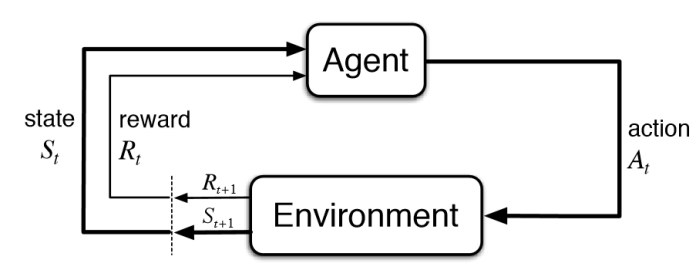
\includegraphics[width=10cm]{supervised reinforcement learning}
	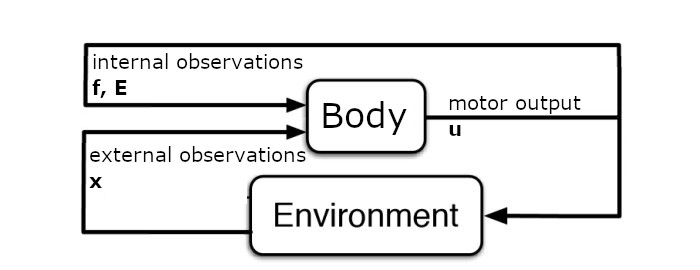
\includegraphics[width=10cm]{unsupervised reinforcement learning}
	\caption{Comparison of supervised (top) and unsupervised (bottom) reinforcement learning}
	\label{fig:rl}
\end{figure} 

If the agent builds an internal model of the world, that works like a map, it could then use such cognitive map to very quickly and efficiently search for energy sources. This only requires imagination, which is much cheaper than locomotion. The ECC networks do not see any reward. Instead, when the energy increases, certain neurons become temporarily more plastic than usually. This mechanism could be used to bias the cognitive map more towards places and actions that lead to the source of energy.

Once the agent has an internal map, it could then exactly know which aspects of the environment are unexplored. Unlike in the current deep reinforcement learning approaches, an agent with episodic memory would only need to visit a novel place once in order to learn about it. If the world is dynamically changing, then an attention mechanism will be necessary. If an animal sees or hears something unexpected it will focus all its attention on the novel experience. This mechanism can be explained using ECC networks as well. Suppose that the current internal model $\boldsymbol{y}$ explains all the previously experienced observations $p(\boldsymbol{x})=\sum_j p(\boldsymbol{x},y_j)$. If the agent experiences something novel that does not fit into any specific $y$, then it will be surprised. The agent will become curious and focus on the novel experience for a while. After the model  $\boldsymbol{y}$ restructures itself and learns about the new $\boldsymbol{x}$, then the agent becomes ``bored''. 

\section{Optimisations and efficiency benchmarks}

\paragraph{Optimisations}
Sparsity enables major optimisations. We can define ECC layers with thousands of neurons, leading to $W$ matrices with millions of weights. Computing them is cheap and can be done on a single CPU because the input vector is sparse and binary. We do not need to multiply $\boldsymbol{x}W$ entirely. If we represent $\boldsymbol{x}$ as a list of indices of active neurons, then we can only iterate such list and visit only a handful of columns in $W$. The $\argmax$ operation is linear. During learning we have to renormalise the winning column of $W$. This requires computing sum, which is of linear complexity. We can achieve constant complexity if we implement a stochastic algorithm, that is, we add $\epsilon$ to $w_{ik}$ for $x_i=1$ (this operation is constant because $\boldsymbol{x}$ is sparse) and then we randomly choose a few other $w_{ik}$ for $x_i=0$ and subtract $\epsilon$ from them. We might need to check if $w_{ik}>0$ in order to avoid introducing negative values. This ensures that weights always sum up to $1$.

\paragraph{Benchmarks}
We ran benchmarks on random patches of MNIST images. Each patch was 25x25 pixels. The network had 734400 learnable parameters (and several non-learnable sparse matrices). Our implementation written in Rust was able to process 2000 images per second on a single thread on 2.7 GHz Intel i5 core. When learning was enabled, it could train on 1700 images per second.

\section{Inhibitory plasticity}

In the original definition, all of the excitatory neurons that share a common inhibitory one, are mutually exclusive. This is an abstraction that simplifies the biological mechanisms.
In reality the inhibitory neurons themselves are plastic and there exist special hebbian learning rules for them, called inhibitory long term potentiation (iLTP). It is possible to provide alternative implementation of ECC networks in a way that uses iLTP. 

\paragraph{Problems of ECC networks}
There are two problems in ECC networks that iLTP could solve at once. One of them is the question of what happens when one excitatory neuron in connected to two inhibitory. Then it will be mutually exclusive with two populations and as a result, it will fire significantly less often then any of its neighbours. Figure \ref{fig:inh_problem} provides an example.
 
 \begin{figure}[!htbp]
 	\centering
 	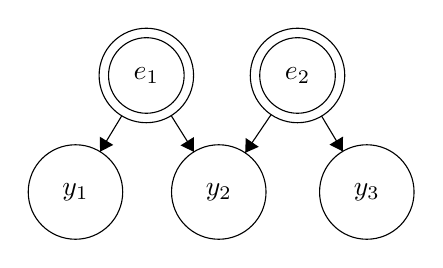
\begin{tikzpicture}[scale=0.2]
 		\tikzstyle{every node}+=[inner sep=0pt]
 		\draw [black] (23.6,-17) circle (3);
 		\draw (23.6,-17) node {$y_1$};
 		\draw [black] (32.7,-17) circle (3);
 		\draw (32.7,-17) node {$y_2$};
 		\draw [black] (42.1,-17) circle (3);
 		\draw (42.1,-17) node {$y_3$};
 		\draw [black] (28.1,-9.6) circle (3);
 		\draw (28.1,-9.6) node {$e_1$};
 		\draw [black] (28.1,-9.6) circle (2.4);
 		\draw [black] (37.7,-9.6) circle (3);
 		\draw (37.7,-9.6) node {$e_2$};
 		\draw [black] (37.7,-9.6) circle (2.4);
 		\draw [black] (26.54,-12.16) -- (25.16,-14.44);
 		\fill [black] (25.16,-14.44) -- (26,-14.01) -- (25.15,-13.49);
 		\draw [black] (29.68,-12.15) -- (31.12,-14.45);
 		\fill [black] (31.12,-14.45) -- (31.12,-13.51) -- (30.27,-14.04);
 		\draw [black] (36.02,-12.09) -- (34.38,-14.51);
 		\fill [black] (34.38,-14.51) -- (35.24,-14.13) -- (34.41,-13.57);
 		\draw [black] (39.23,-12.18) -- (40.57,-14.42);
 		\fill [black] (40.57,-14.42) -- (40.59,-13.48) -- (39.73,-13.99);
 	\end{tikzpicture}
 	\caption{Suppose $s_1<s_2<s_3$. Then $y_1$ won't be able to fire, because $y_2$ has higher $s_2$. Unfortunately $y_2$ also is unable to fire because it loses against $y_3$. As a result none of the neurons connected to $e_1$ fires. The same problem appears when $s_1>s_2>s_3$. As a result the probability of $y_2$ becoming active is significantly lower than that of its neighbours.}
 	\label{fig:inh_problem}
 \end{figure} 

The second problem is concerned with biological plausibility. In all of the ECC topologies presented so far, the ratio of inhibitory to excitatory neurons is around 1 to a few dozen or hundred. In the real brain, inhibitory neurons make up about 20\%. This leads to an efficiency problem. Currently the pattern of inhibition is fixed and a single neuron would need to send its inhibitory neurotransmitter to all of the excitatory neurons. It should be noted that most of the time, a given input pattern $\boldsymbol{x}$ will significantly potentiate ($s$ value will be high) only for a small fraction of $\boldsymbol{y}$ neurons. It would be more efficient to first look at the pattern in  $\boldsymbol{x}$ and then send the inhibitory  neurotransmitters only to those $y$ that we expect to fire the most.

\paragraph{Plastic inhibitory neurons}
Both of the problems are solved by introducing more inhibitory neurons and allowing them to choose their connections via plasticity mechanisms. Instead of using $\argmax$, every neuron should have a spiking threshold. The inhibitory neurons $\boldsymbol{el}$are excited by the same (or similar) inputs $\boldsymbol{x}$ as the excitatory $\boldsymbol{y}$. When a neuron $y_j$ is depolarised ($s_j$ raises ``high enough'') but does not fire ($s_j$ is below the threshold) after $e_k$, then the synapse from $e_k$ to $y_j$ is strengthened. 

\section{ECC are spiking networks}

The ECC can be extended to work with time series, model sequential data, detect movement and distance of objects. Let $\boldsymbol{x}^{(t)}$ and $\boldsymbol{y}^{(t)}$ be the input signal and states of neurons at time step $t$ respectively. We can concatenate several such vectors $\boldsymbol{x}^{(t-b)}\cdot \boldsymbol{x}^{(t-b+1) }\cdot ...\cdot\boldsymbol{x}^{(t)}=\boldsymbol{\hat{x}}^{(t)}$ up to $b$ steps from the past. Analogically for $\boldsymbol{\hat{y}}^{(t)}$. Now the weight matrices $W$ can span not only neurons but also their past states. The connections are now made not only across space but also time. The size of $W$ is given by $bnm$ where $n$ and $m$ is the number of input $\boldsymbol{x}$ and hidden $\boldsymbol{y}$ neurons respectively. The memory complexity is therefore cubic. There is a certain heuristic that can be exploited in order to obtain a quadratic complexity. The natural environment is time-consistent, meaning that usually $\boldsymbol{x}$ only changes a little between time steps. When the agent is idle, it may look in a specific direction for prolonged period of time and always observe the same $\boldsymbol{x}$. Therefore we could agree to only make one connection to a specific point in time per input-output pair. Hence the matrix $W$ is not a Cartesian product $[t-b,t] \times \boldsymbol{x} \times \boldsymbol{y} \rightarrow [0,1]$  but rather a function $\boldsymbol{x} \times \boldsymbol{y} \rightarrow [t-b,t] \times [t-b,t] \times [0,1]$ where $[t-b,t] \times [t-b,t]$ are the beginning and end of the time-window (relative to current time $t$).

In the case of continuous time, primitive distributions must be represented using a different data structure than a matrix. The dendrites of biological neurons carry their information at different speeds. The faster dendrites connect to recent past, whereas slower ones detect signal from to more distant past. The action potential doesn't vanish instantly. A plateau potential may linger for a certain period of time, which means that the neuronal connections can be tuned to a time-interval of some specific length. The neurons tend to fire in spike trains of specific frequency. Two subsequent spikes coming from the same input are likely correlated and do not carry additional information, hence it's pointless to have multiple connections to the same input tuned to distinct times. This again allows for reducing the complexity from cubic to quadratic. Hence the optimal data structure for representing continuous primitive distributions is a function $\boldsymbol{x} \times \boldsymbol{y} \rightarrow \mathbb{R} \times \mathbb{R} \times [0,1]$ where $\mathbb{R} \times \mathbb{R}$ represents beginning and end of time interval.

The standard ECC learning algorithm can be used to train $W$ matrices of cubic complexity. When we used the heuristic quadratic $W$, then the spike-time-dependent plasticity emerges as the optimal learning method. If the input spike comes too early, we move the time window a little to the past. If it comes too late, we move it a notch to the future. If the variance of relative spike time is high, then we stretch the time window to be longer. If the input arrives at a very predictable time, then we can narrow down the window size. 

The dendrites of biological neurons are arranged in a tree-like structure. Tuning the time-window selectivity of the dendrite will affect all of the synapses. Under such circumstances, the only way to fine-tune individual synapses is to disconnect them if the time-window of the current dendrite is unsuitable and hope that some other dendrite happens to be better tuned and could form the right synapses.	


\section{Evolving ECC networks}

The receptive fields $p(\boldsymbol{x},y_j)$ of neurons are primarily driven by their respective topologies $\tau$. We can embed the set of all neurons $\boldsymbol{y}$ in a n-dimensional euclidean space. This way we obtain a norm on all nodes in the graph. Neurons that are in close proximity, should have higher probability of developing similar topologies. Then the task of evolving ECC network becomes reduced to evolution of manifolds in a euclidean space. Kenneth Stanley's ES-HyperNEAT algorithm can be repurposed for such a task. 



\bibliographystyle{BibTeXtran}   % (uses file "BibTeXtran.bst")
\bibliography{BibTeXrefs}    







\end{document}
